\chapter{RESULTS AND ANALYSIS}

%  WRITING GUIDELINES FOR RESULTS AND ANALYSIS CHAPTER
%  ====================================================
% The Results and Analysis chapter presents the outcomes of your project and critically analyzes
% them. This chapter demonstrates whether your system meets requirements, compares performance
% against objectives and baselines, and interprets findings. Results should be presented objectively
% with appropriate visualizations, while analysis provides context and explanation. This chapter should be full of charts, tables, and figures illustrating your system's performance and behaviour.


% %  LaTeX quick refs:
% \begin{itemize}
%     \item Always reference figures and tables in the text before they appear.
%     \item Use the cleveref package; write \verb|\cref{fig:label}| or \verb|\Cref{tab:label}| for automatic formatting (add \verb|\usepackage{cleveref}| to the preamble).
%     \item Keep captions descriptive and use unique labels per chapter (e.g., \texttt{fig:my-figure}, \texttt{tab:results}).
% \end{itemize}

\section{Comparative Analysis of Object Detection using YOLOv5 and YOLOv7}

\subsection{Experimental Setup}

A comparative study using \gls{yolo}v5 and \gls{yolo}v7 to detect and classify hand-drawn electronic circuit components was conducted to determine which model is better-suited for the needs of this project. The dataset consisted of 61 classes, including resistors, capacitors (polarized and unpolarized), diodes, transistors (\gls{bjt} and \gls{fet}), integrated circuits, switches, and more. To ensure a fair comparison, both models were trained and validated on identical data splits.

\subsection{Training Progress and Loss Curves}

While training, loss metrics (bounding box loss, objectness loss, and the classification loss) were tracked. The training curves show how these metrics evolved over time. No substantial difference was seen between the loss metrics of \gls{yolo}v5 and v7.

\begin{figure}[H]
    \centering
    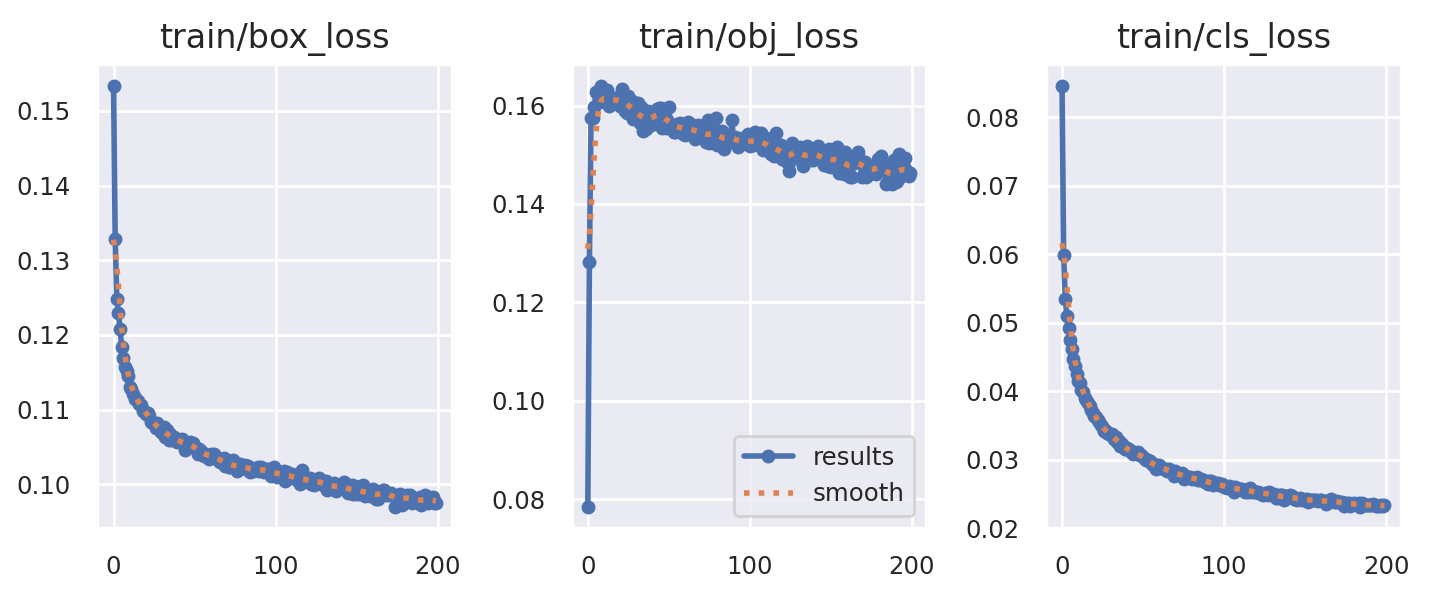
\includegraphics[width=\textwidth]{src/images/figures/loss_curve_yolov5.png}
    \caption{Loss Curves for YOLOv5}
    \label{fig:yolov5-loss-curves}
\end{figure}

\begin{figure}[H]
    \centering
    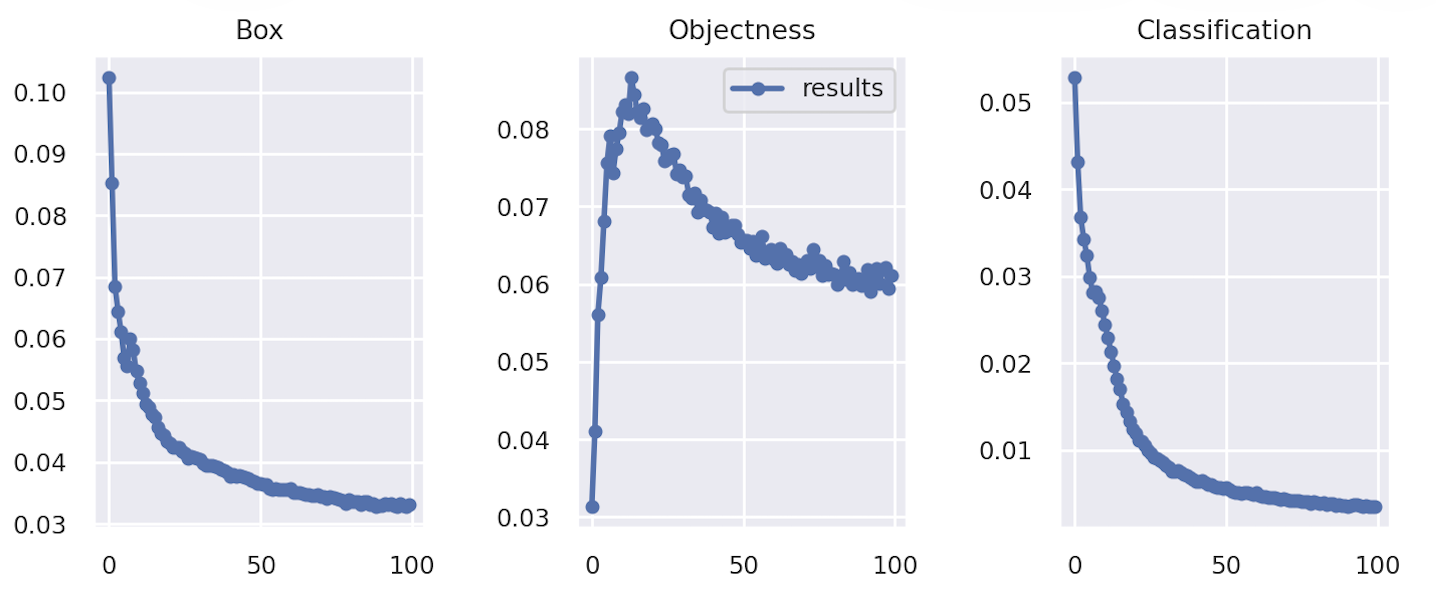
\includegraphics[width=\textwidth]{src/images/figures/loss_curve_yolov7.png}
    \caption{Loss Curves for YOLOv7}
    \label{fig:yolov7-loss-curves}
\end{figure}

\subsection{Performance Metrics}

\subsubsection{mAP vs Number of Epochs}

In order to monitor the progress in models' ability to recognize components as the training progressed, both \gls{map}@0.5 and \gls{map}@0.5:0.95 were plotted across all epochs. These curves depict how quickly and effectively each model learns over time.

\begin{figure}[H]
    \centering
    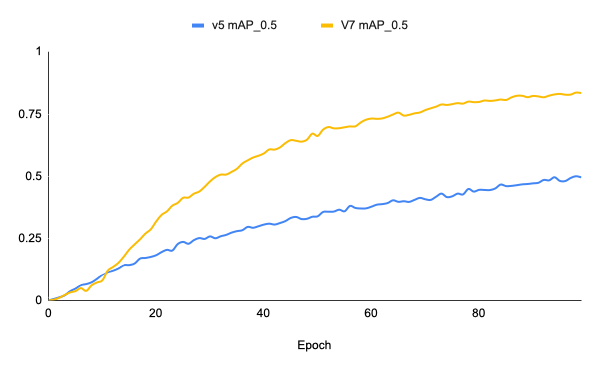
\includegraphics[width=\textwidth]{src/images/figures/map_vs_epochs.png}
    \caption{\gls{map}@0.5 vs Epochs for YOLOv5 and YOLOv7}
    \label{fig:map50-epochs}
\end{figure}

\begin{figure}[H]
    \centering
    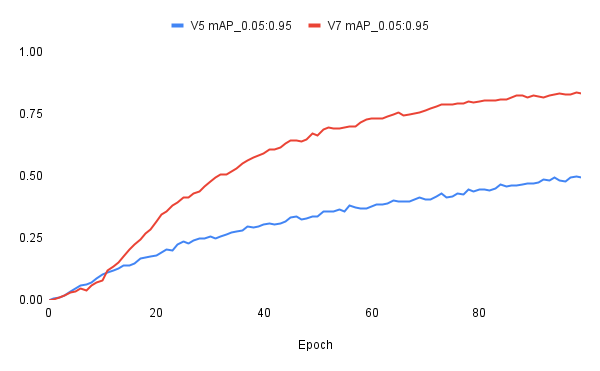
\includegraphics[width=\textwidth]{src/images/figures/map_vs_epochs_0.5to0.95.png}
    \caption{\gls{map}@0.5:0.95 vs Epochs for YOLOv5 and YOLOv7}
    \label{fig:map50-95-epochs}
\end{figure}

It is clear from both \cref{fig:map50-epochs} and \cref{fig:map50-95-epochs} that the \gls{map} scores for \gls{yolo}v7 are significantly better than that for \gls{yolo}v5. Likewise, the loss curves, as shown in \cref{fig:yolov5-loss-curves,fig:yolov7-loss-curves}, demonstrate a steeper curve in the case of YOLOv7.

\subsubsection{Precision, Recall, and F1 Score vs Confidence}

The following graphs demonstrate the model performance under varying confidence thresholds:

\paragraph{Precision vs Confidence}

\begin{figure}[H]
    \centering
    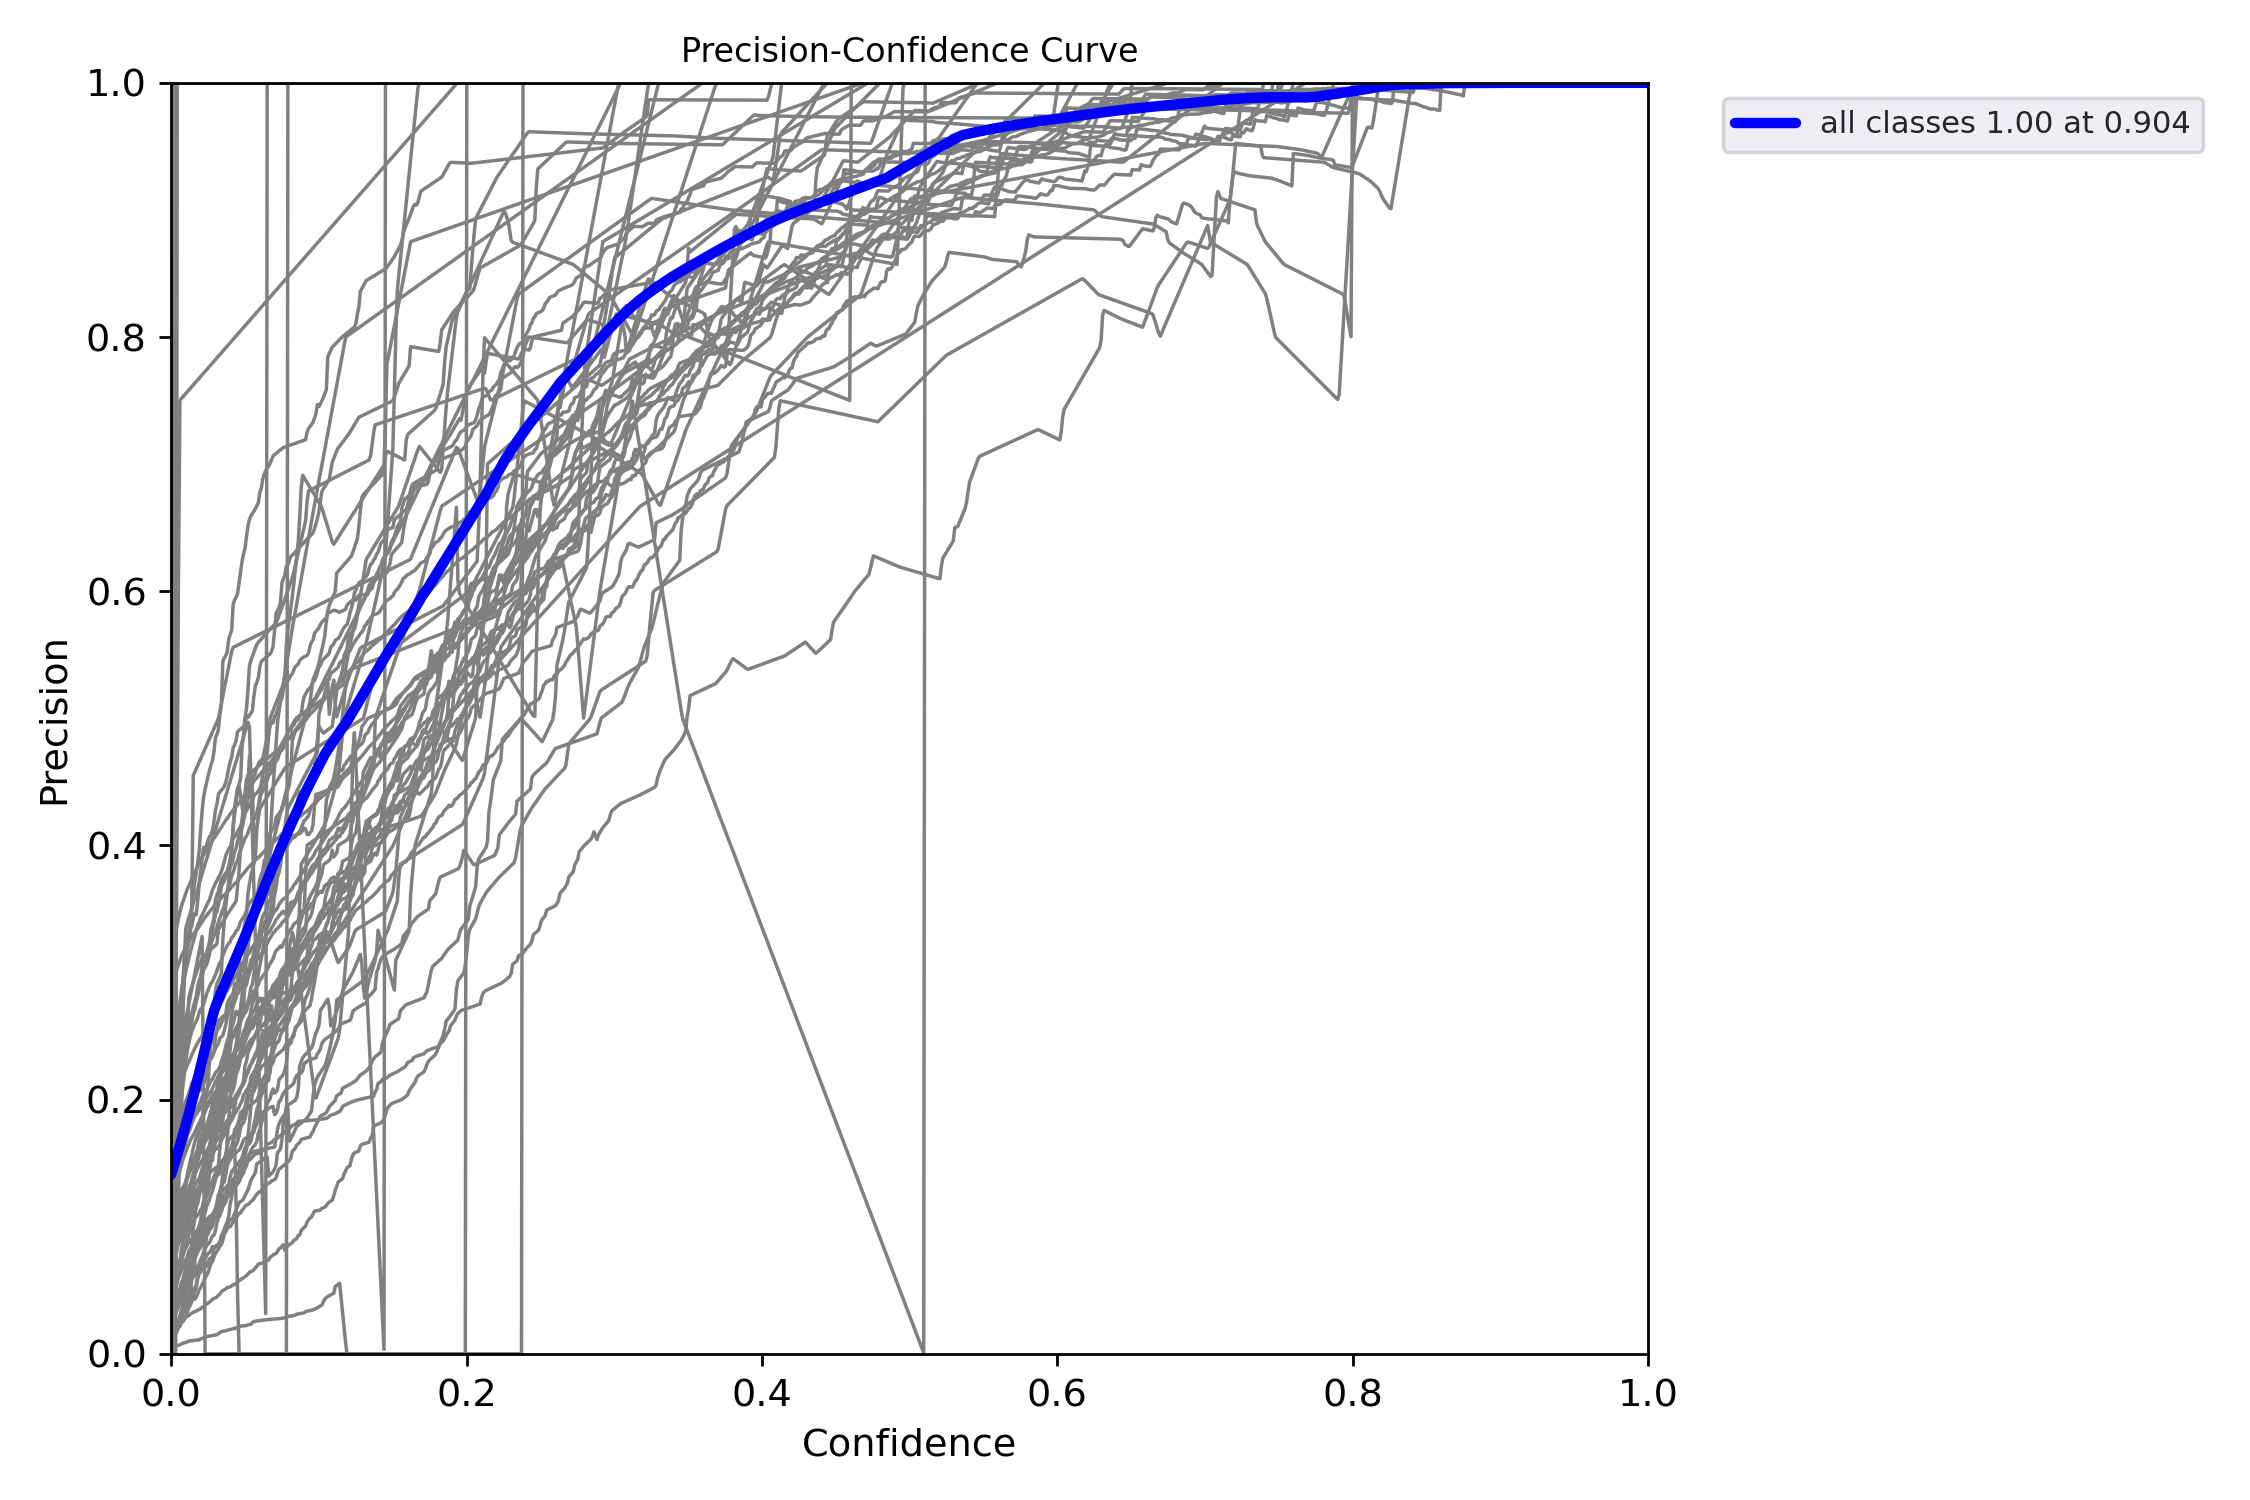
\includegraphics[width=\textwidth]{src/images/figures/precision_vs_confidence_yolov5.png}
    \caption{Precision-Confidence Curve for YOLOv5}
    \label{fig:precision-conf-v5}
\end{figure}

\begin{figure}[H]
    \centering
    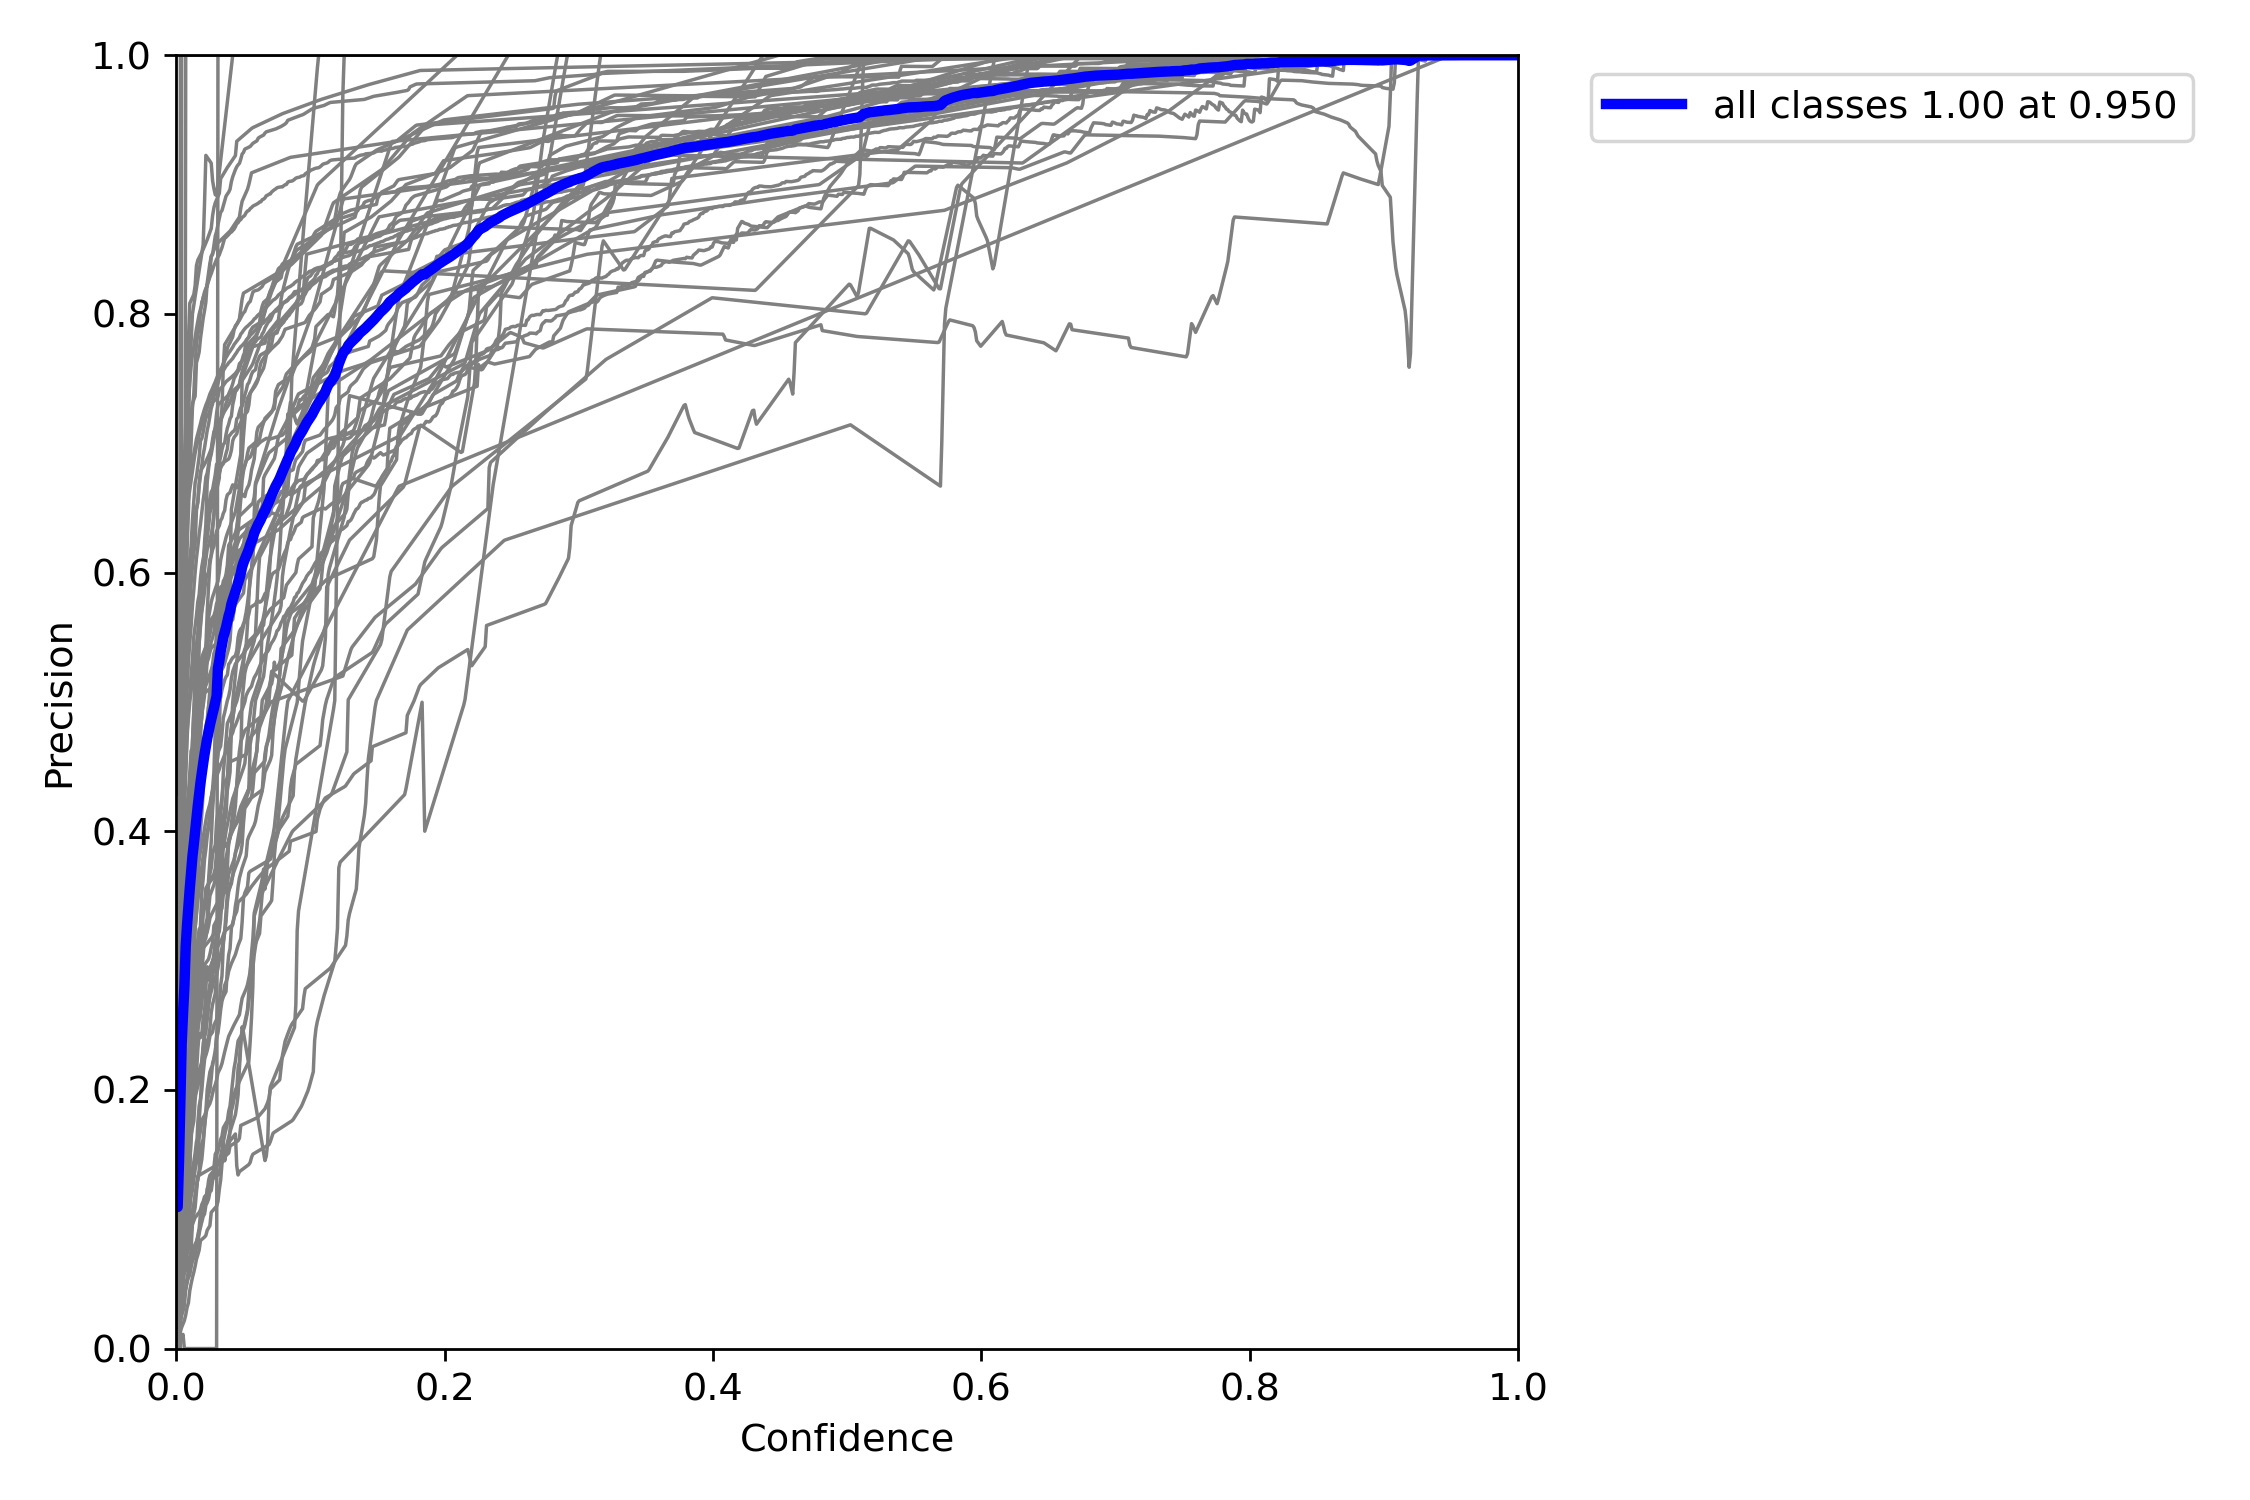
\includegraphics[width=\textwidth]{src/images/figures/precision_vs_confidence_yolov7.png}
    \caption{Precision-Confidence Curve for YOLOv7}
    \label{fig:precision-conf-v7}
\end{figure}

\cref{fig:precision-conf-v5} and \cref{fig:precision-conf-v7} demonstrate the Precision-Confidence Curve for YOLOv5 and YOLOv7 respectively. The area under this curve informs how consistently precise the model is across all confidence thresholds. For a large area under the curve, as in the case of YOLOv7, the model maintains good precision even when threshold changes; however, for a smaller area, precision collapses quickly when threshold is relaxed.

\paragraph{Recall vs Confidence}

\begin{figure}[H]
    \centering
    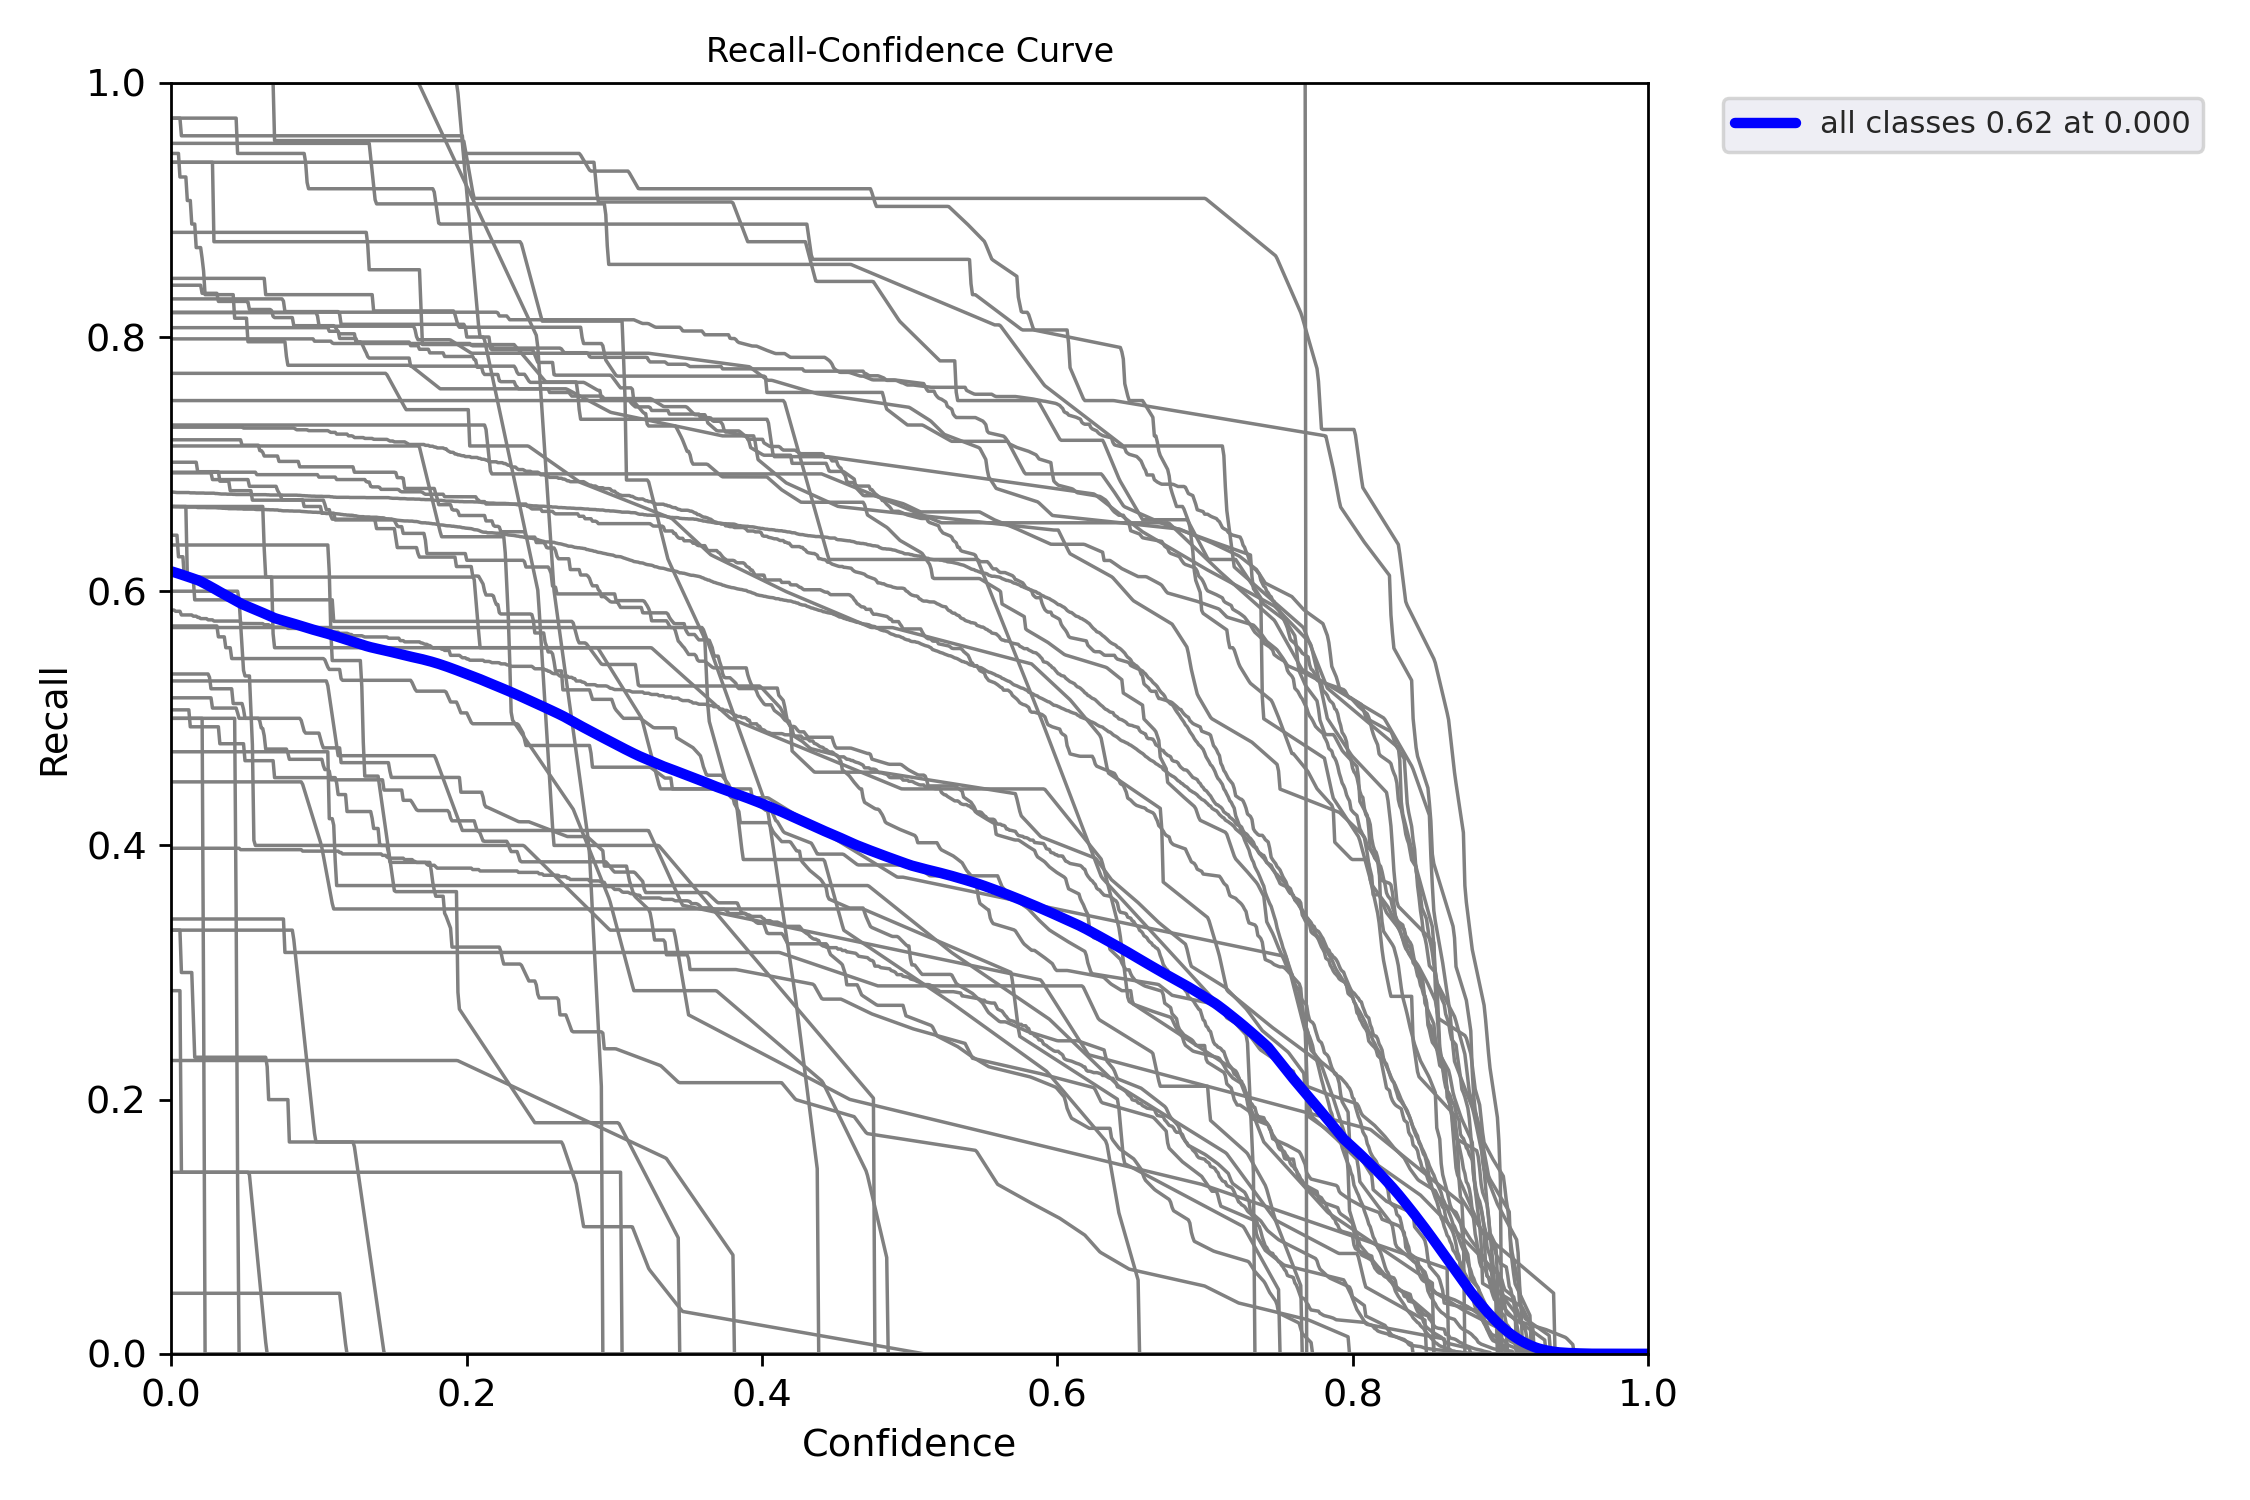
\includegraphics[width=\textwidth]{src/images/figures/recall_vs_confidence_yolov5.png}
    \caption{Recall-Confidence Curve for YOLOv5}
    \label{fig:recall-conf-v5}
\end{figure}

\begin{figure}[H]
    \centering
    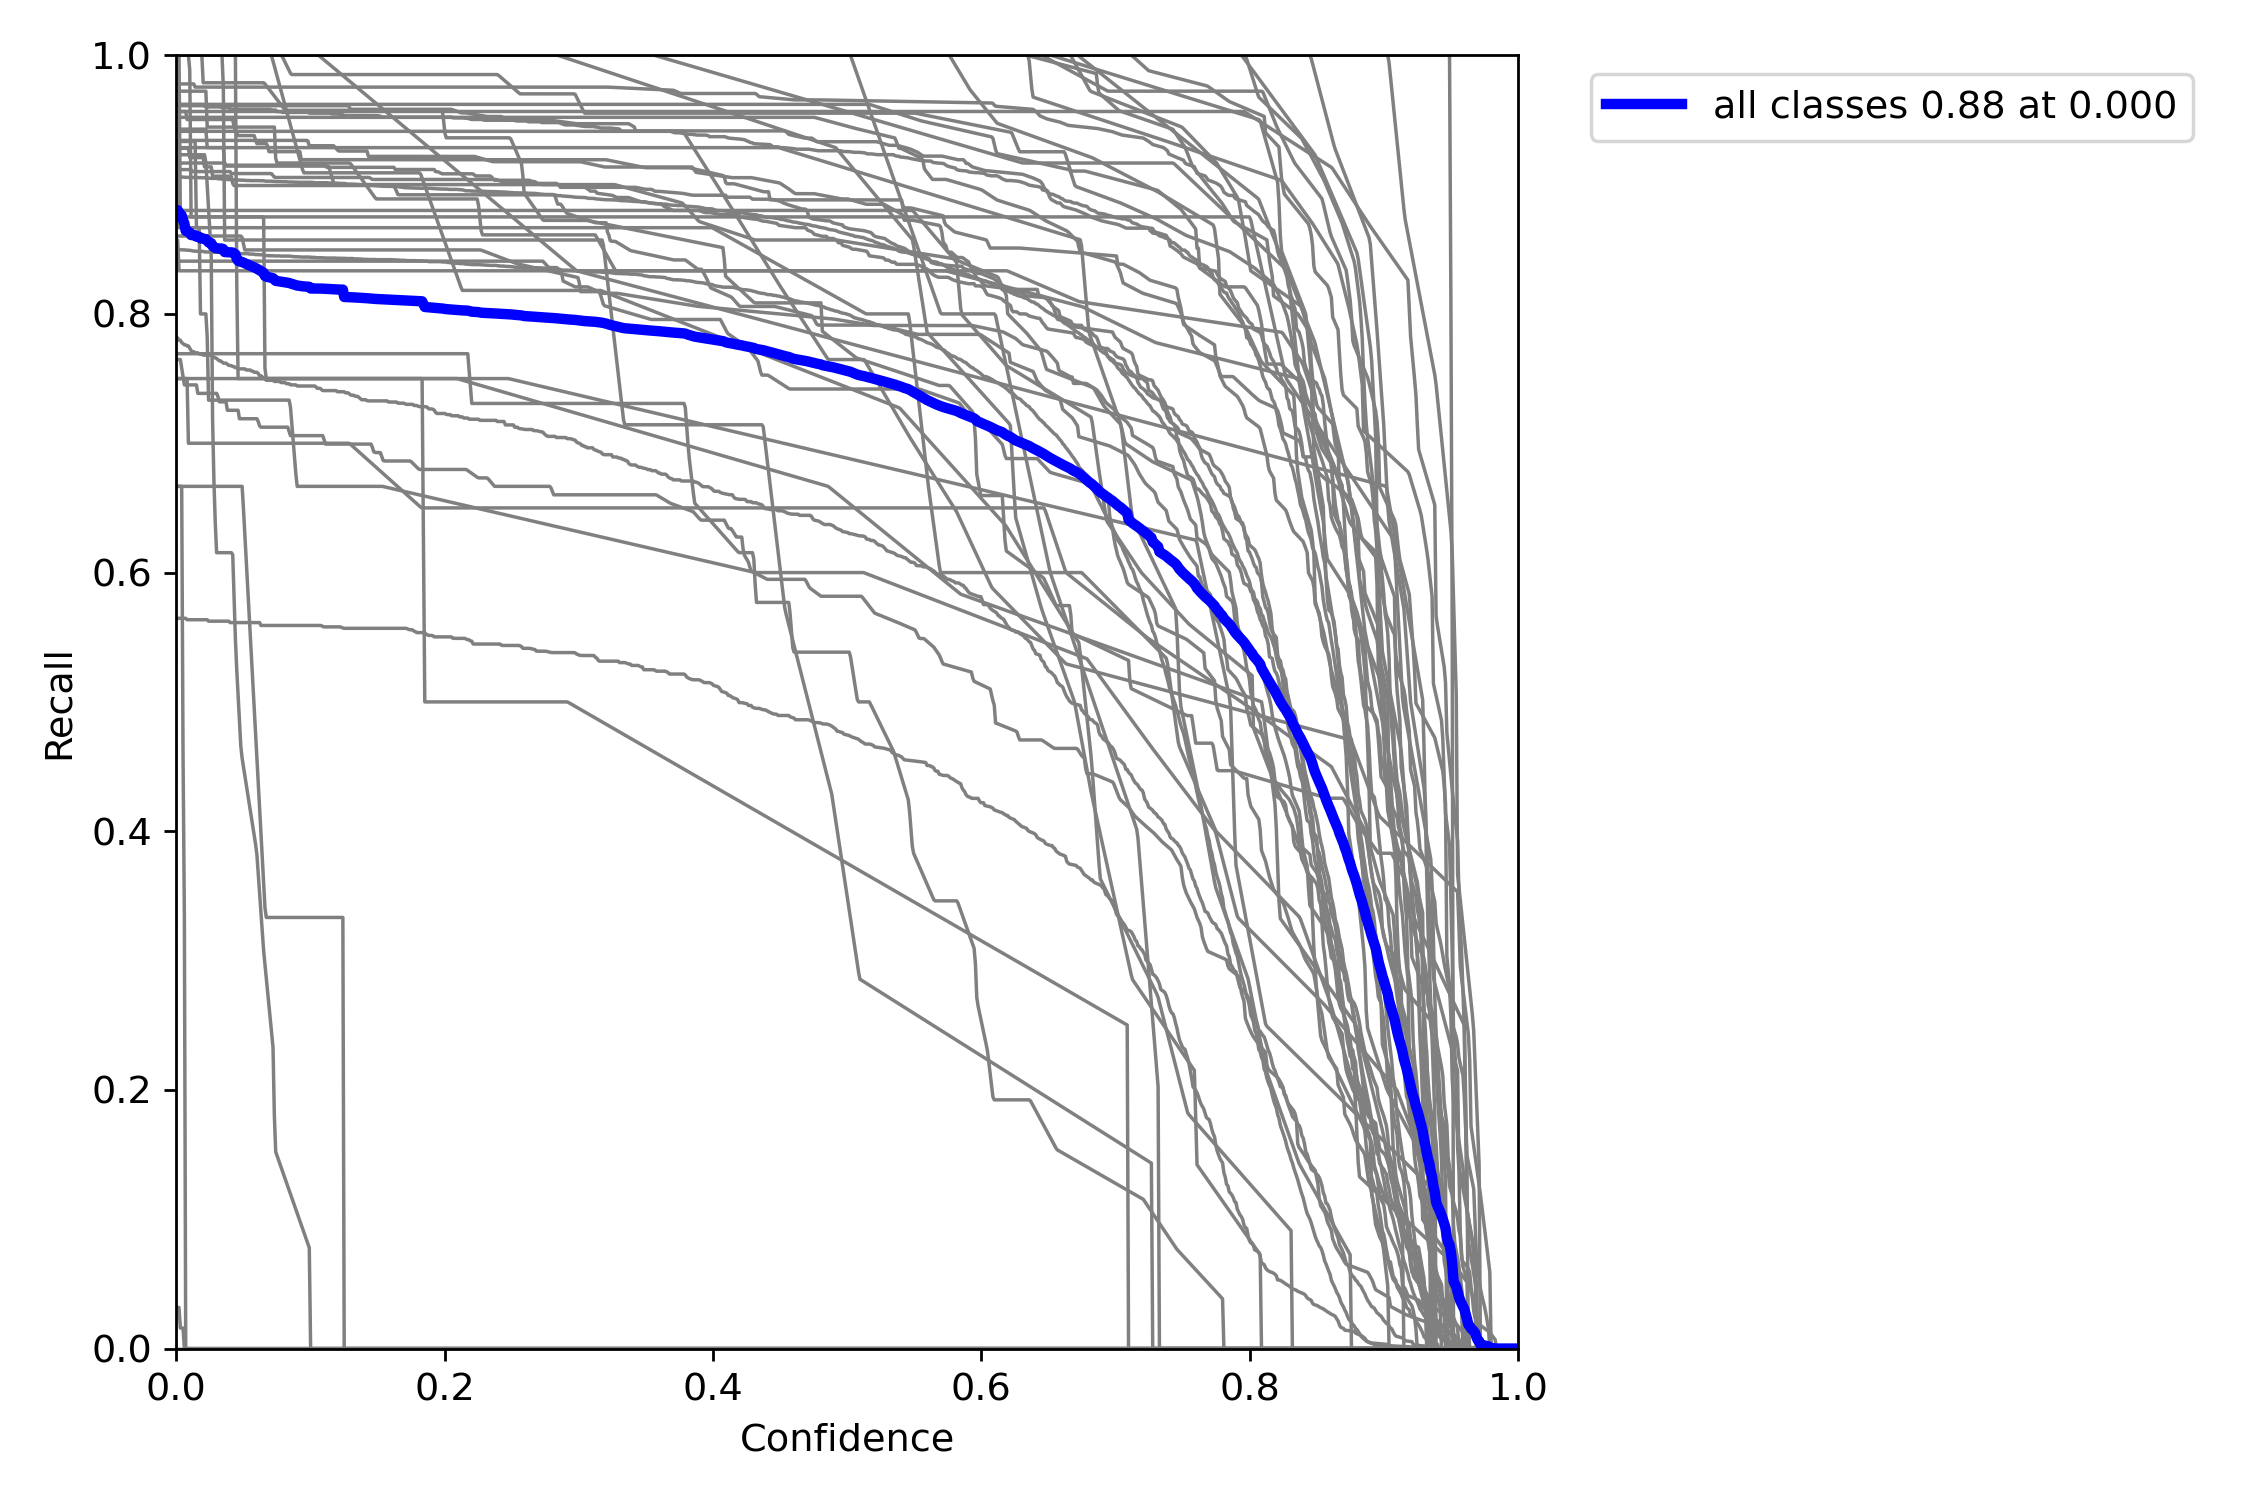
\includegraphics[width=\textwidth]{src/images/figures/recall_vs_confidence_yolov7.png}
    \caption{Recall-Confidence Curve for YOLOv7}
    \label{fig:recall-conf-v7}
\end{figure}

\cref{fig:recall-conf-v5} and \cref{fig:recall-conf-v7} demonstrate the Recall-Confidence Curve for YOLOv5 and YOLOv7 respectively. The area under this curve informs how well the model preserves recall while increasing certainty. For a large area, the recall stays high even with strict thresholds.

\paragraph{F1 Score vs Confidence}

\begin{figure}[H]
    \centering
    \includegraphics[width=\textwidth]{src/images/figures/f1_vs_confidence_yolov5.png}
    \caption{F1 Score-Confidence Curve for YOLOv5}
    \label{fig:f1-conf-v5}
\end{figure}

\begin{figure}[H]
    \centering
    \includegraphics[width=\textwidth]{src/images/figures/f1_vs_confidence_yolov7.png}
    \caption{F1 Score-Confidence Curve for YOLOv7}
    \label{fig:f1-conf-v7}
\end{figure}

\cref{fig:f1-conf-v5} and \cref{fig:f1-conf-v7} demonstrate the F1 Score-Confidence Curve for YOLOv5 and YOLOv7 respectively. The larger the area under this curve, the higher the robustness of the precision-recall trade-off across thresholds.

\paragraph{Precision-Recall Curve}

\begin{figure}[H]
    \centering
    \includegraphics[width=\textwidth]{src/images/figures/pr_curve_yolov5.png}
    \caption{Precision-Recall Curve for YOLOv5}
    \label{fig:pr-curve-v5}
\end{figure}

\begin{figure}[H]
    \centering
    \includegraphics[width=\textwidth]{src/images/figures/pr_curve_yolov7.png}    
    \caption{Precision-Recall Curve for YOLOv7}
    \label{fig:pr-curve-v7}
\end{figure}

\cref{fig:pr-curve-v5} and \cref{fig:pr-curve-v7} demonstrate the Precision-Recall Curve for YOLOv5 and YOLOv7 respectively. The area under this curve gives the average precision (AP) which informs how good the model is at ranking positive samples above negative ones. The area under each of the curves in these figures is higher for YOLOv7 in comparison to YOLOv5. This is expected behavior and proves YOLOv7 is better than YOLOv5 when it comes to performance. Although YOLOv7 is computationally more intensive and generally heavier than YOLOv5, this is a trade-off willing to be accepted to gain performance.

\subsection{Confusion Matrix}

To assess per-class performance, confusion matrices were generated using the validation set.

\begin{figure}[H]
    \centering
    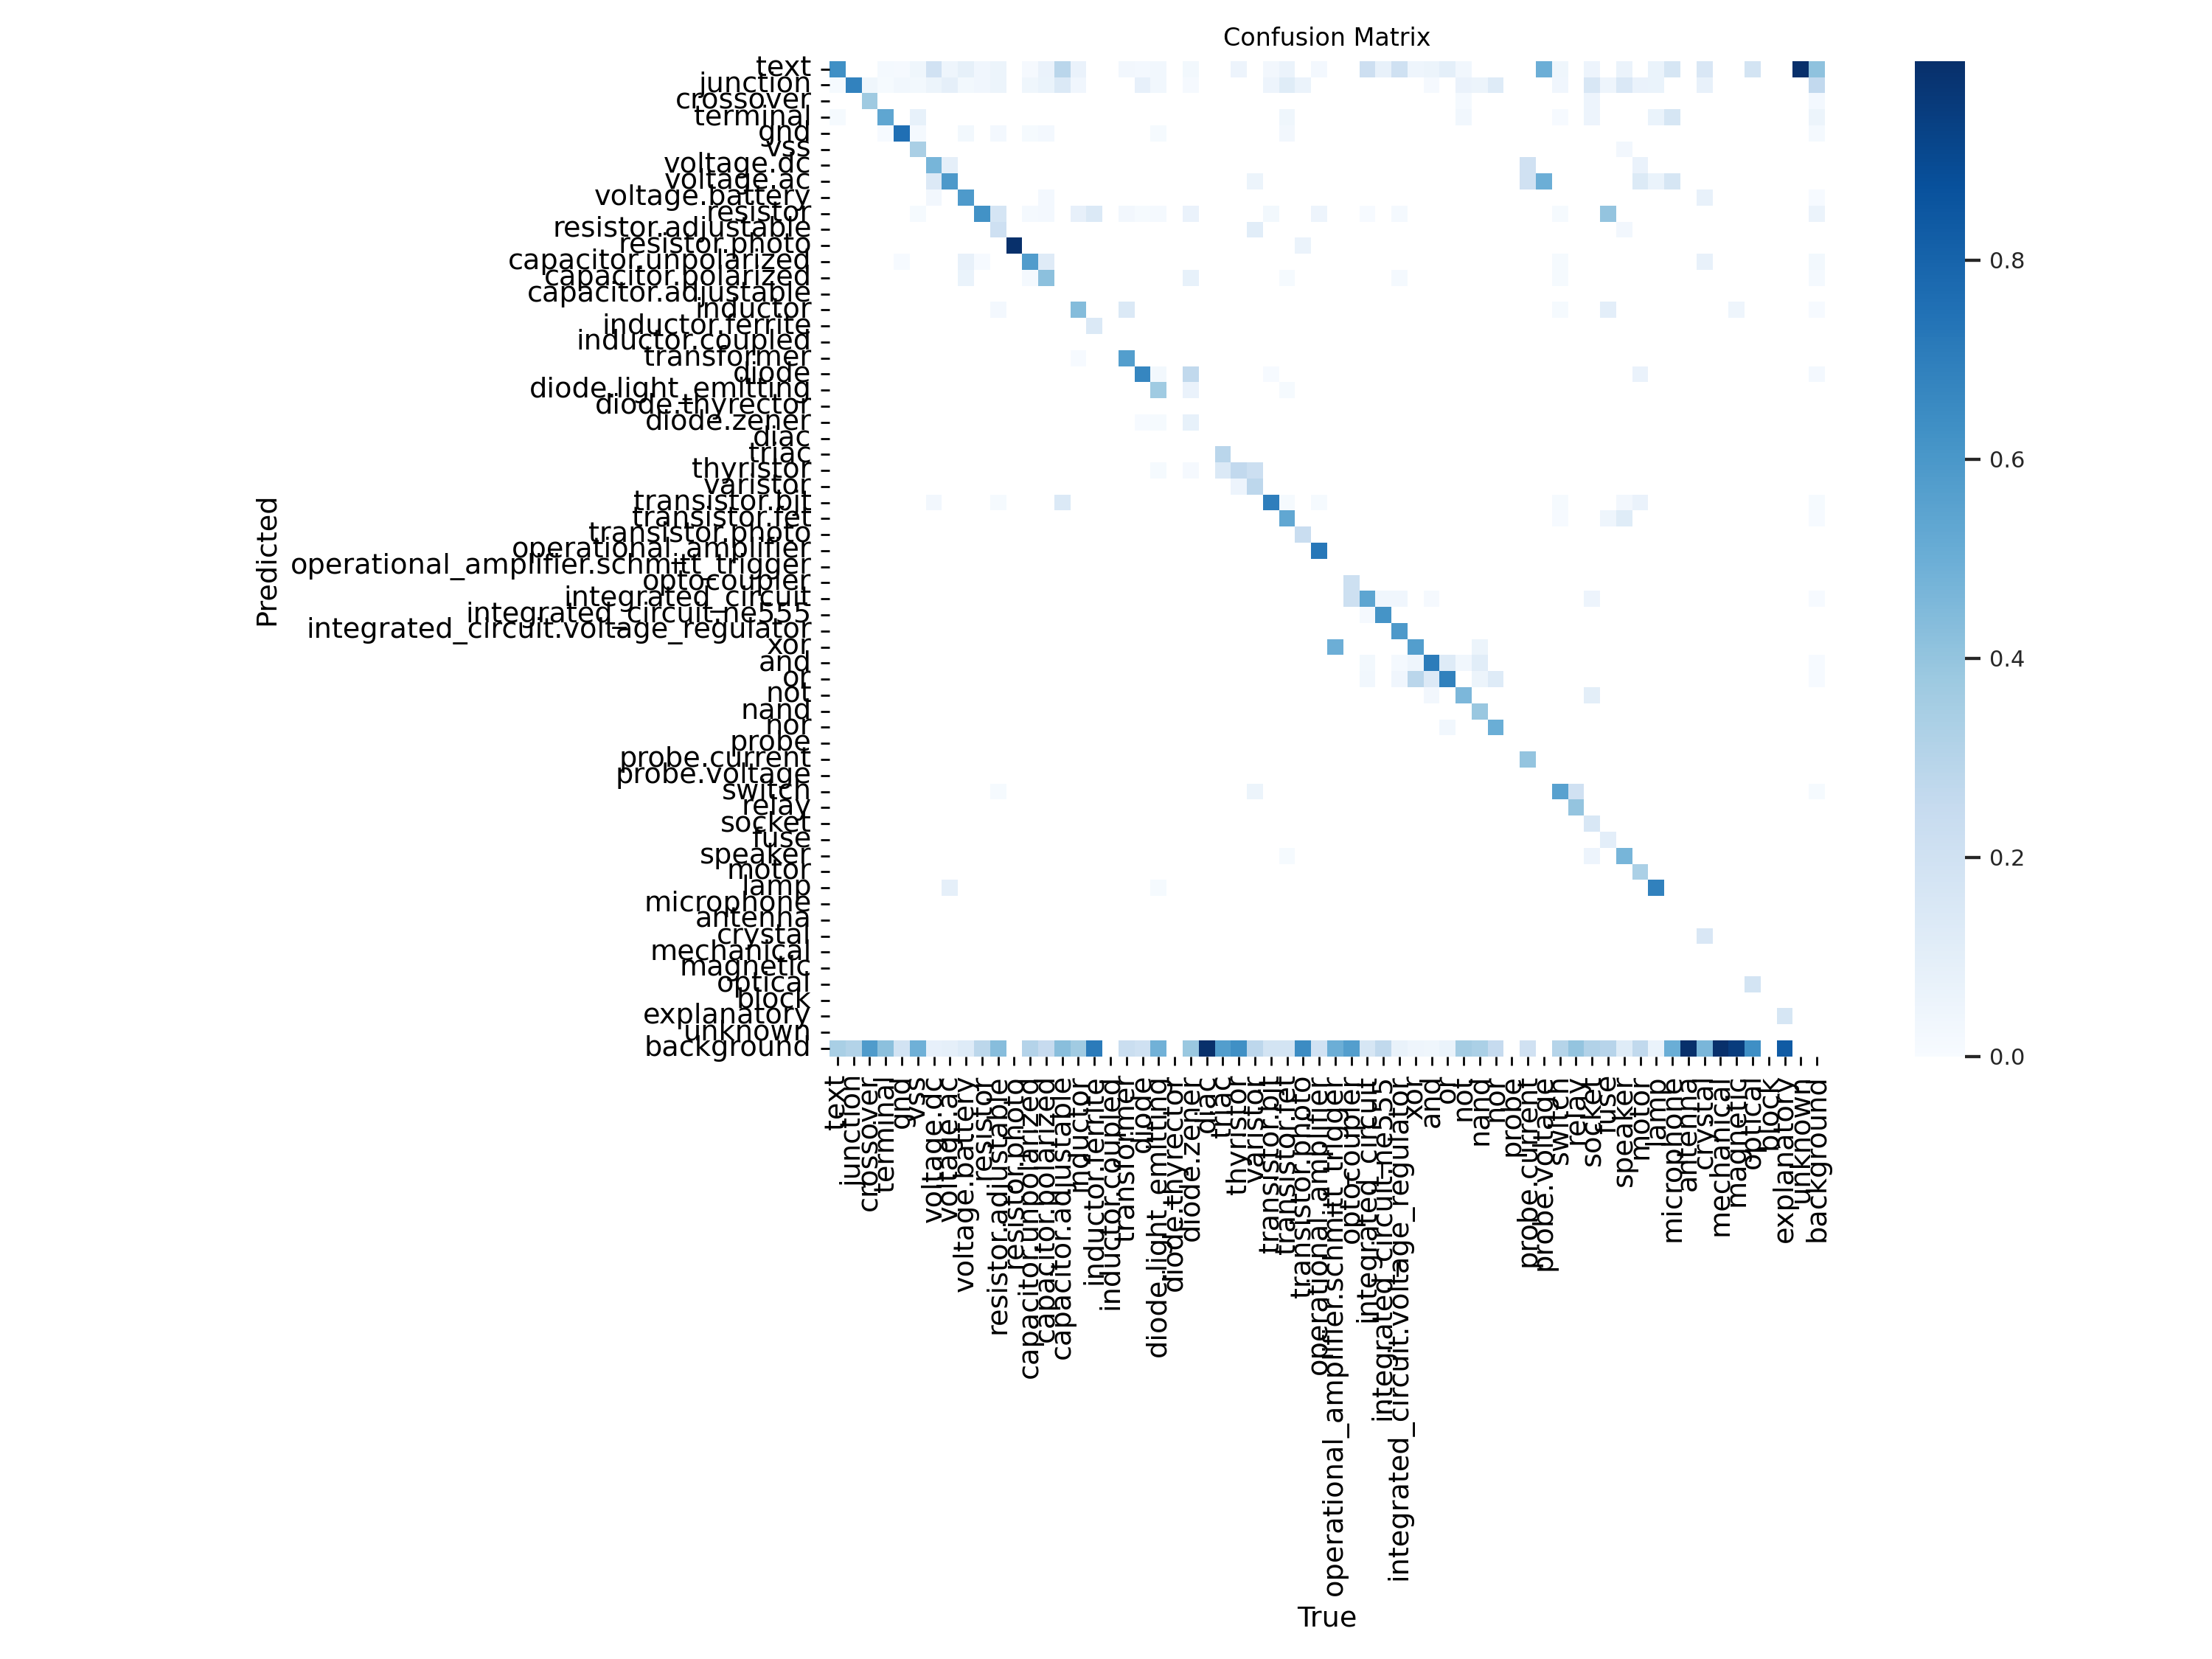
\includegraphics[width=\textwidth]{src/images/figures/confusion_matrix_yolov5.png}
    \caption{Confusion Matrix for YOLOv5}
    \label{fig:confusion-matrix-v5}
\end{figure}

\begin{figure}[H]
    \centering
    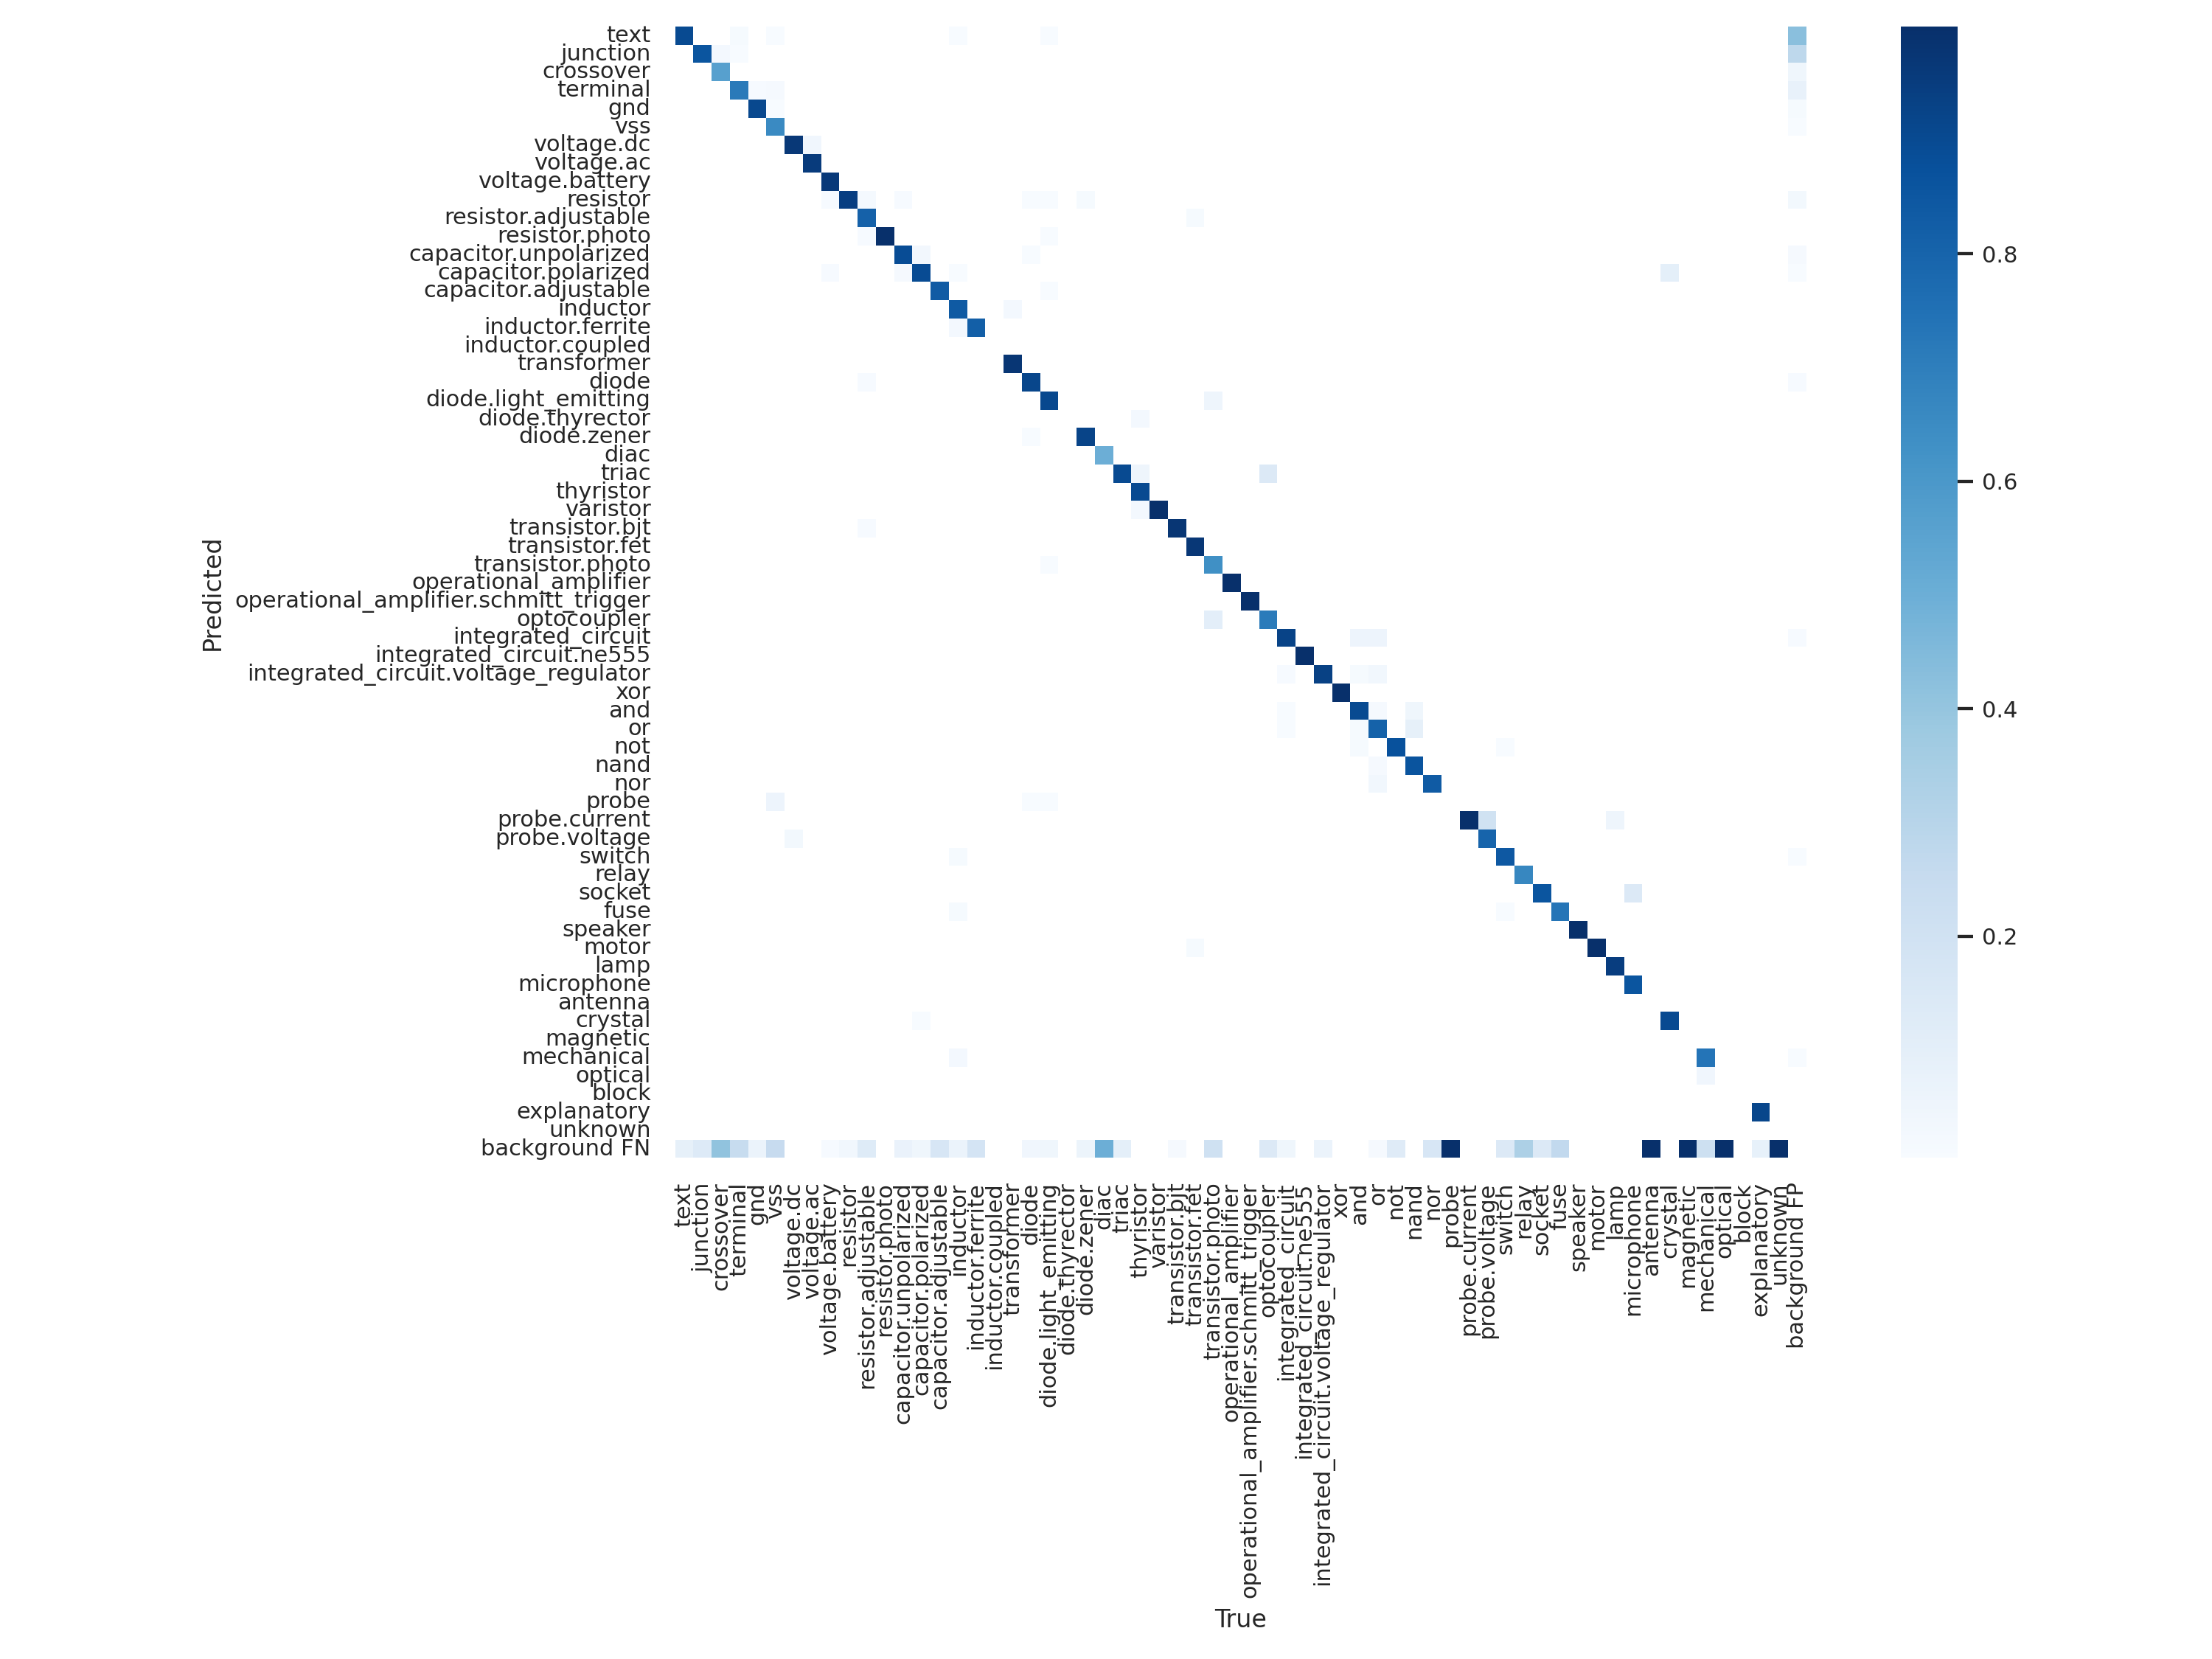
\includegraphics[width=\textwidth]{src/images/figures/confusion_matrix_yolov7.png}    
    \caption{Confusion Matrix for YOLOv7}
    \label{fig:confusion-matrix-v7}
\end{figure}

\cref{fig:confusion-matrix-v5} and \cref{fig:confusion-matrix-v7} demonstrate the confusion matrices for YOLOv5 and YOLOv7 respectively. In comparison, the confusion matrix for YOLOv7 has a very dark main diagonal and very light off-diagonals, which means that the model exhibits strong class separability with minimal inter-class confusion.

\subsection{Quantitative Results Comparison}

Final epoch results show \gls{yolo}v7 outperformed \gls{yolo}v5 across all major metrics.

\begin{table}[H]
    \centering
    \caption{Comparison of Performance Metrics for YOLOv5 and YOLOv7}
    \label{table:yolo-comparison}
    \begin{tabular}{lrr}
        \toprule
        \textbf{Metric} & \textbf{YOLOv5} & \textbf{YOLOv7} \\
        \midrule
        \gls{map}@0.5 & 0.61 & 0.83 \\
        \gls{map}@0.5:0.95 & 0.41 & 0.60 \\
        Precision & 0.84 & 0.93 \\
        Recall & 0.62 & 0.78 \\
        Epochs Trained & 200 & 100 \\
        \bottomrule
    \end{tabular}
\end{table}

Overall, \gls{yolo}v7 showed a clear advantage over \gls{yolo}v5 in our experiments. It not only achieved higher values for precision, recall, and mean average precision but also required fewer epochs to converge. \gls{yolo}v7's confusion matrix reflected better class separation and fewer misclassifications. The improvements in F1 score and overall stability of predictions across confidence thresholds make \gls{yolo}v7 a more robust choice for circuit diagram interpretation.

\section{\gls{ocr} Results}

The out-of-the-box default \gls{easyocr} implementation without fine-tuning was able to detect some of the component values from the circuit; however, the results left a lot to be desired. This made it clear that proper training of the recognition model is absolutely essential for this project.

After training the text recognition model from scratch, results were much improved. Two randomly picked images from the dataset are shown below after passing through the detection (\gls{yolo}v7) and recognition (\gls{ocr}) models.

\begin{figure}[H]
    \centering
    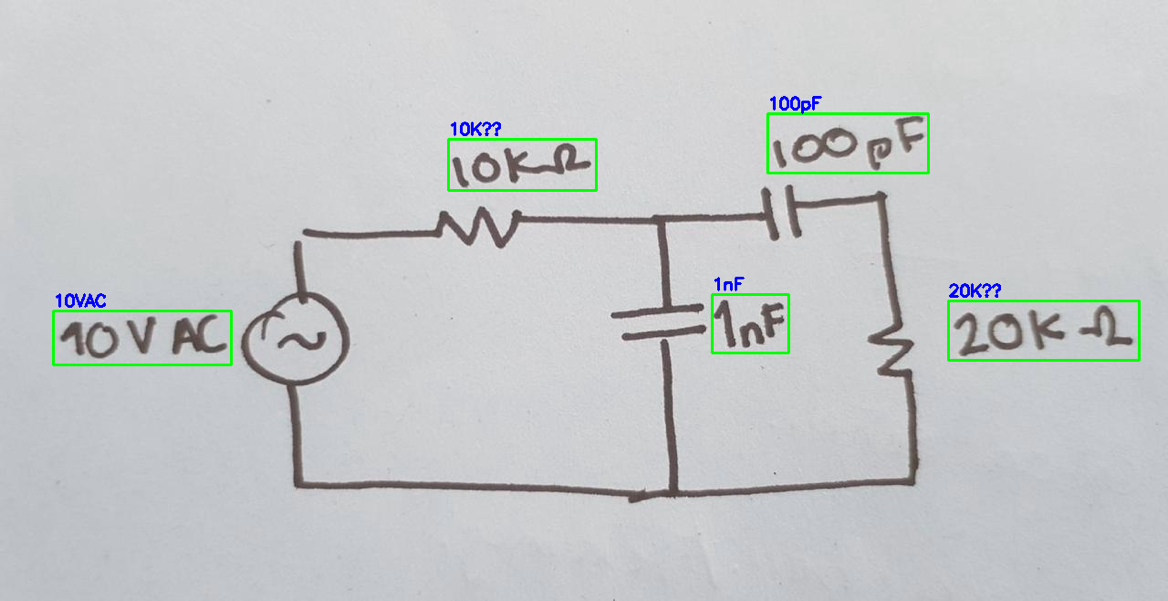
\includegraphics[width=\textwidth]{src/images/figures/text_detection_recognition.png}
    \caption{Text Detection and Recognition (i)}
    \label{fig:ocr-result-1}
\end{figure}

\begin{figure}[H]
    \centering
    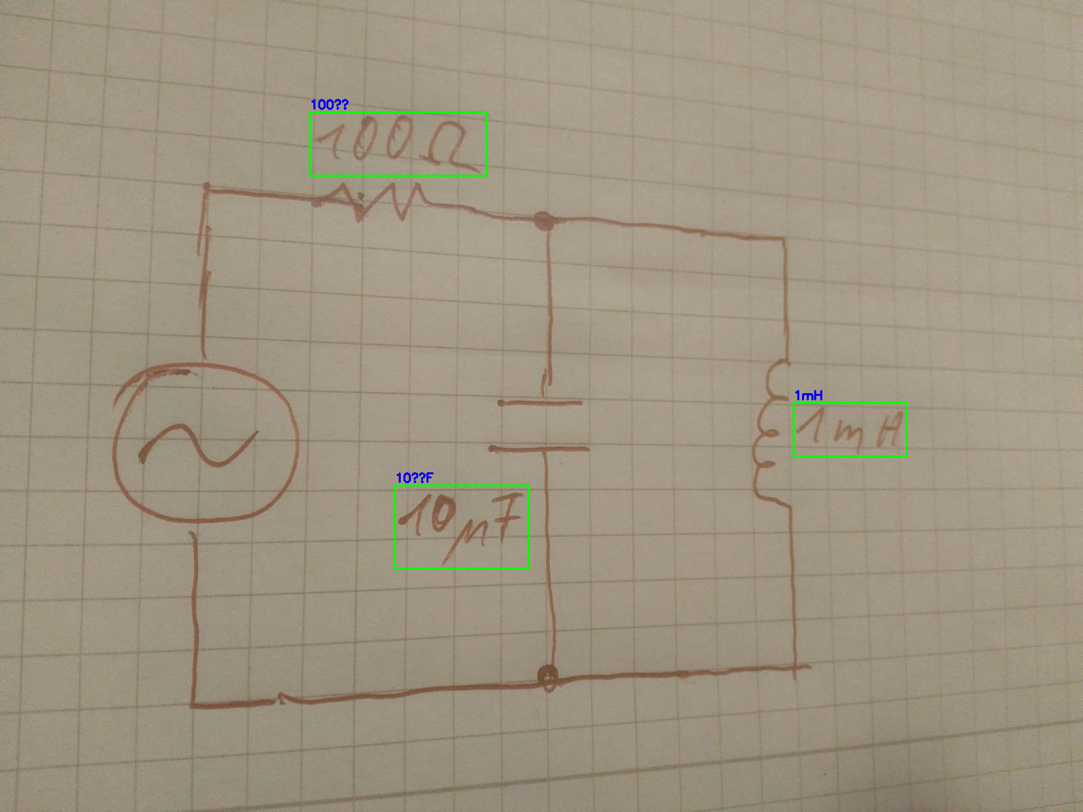
\includegraphics[width=\textwidth]{src/images/figures/text_detection_recognition2.png}
    \caption{Text Detection and Recognition (ii)}
    \label{fig:ocr-result-2}
\end{figure}

It is to be noted that the ``??'' shown in \cref{fig:ocr-result-1} and \cref{fig:ocr-result-2} is a limitation of the picture-rendering library used (OpenCV, Matplotlib), rather than a limitation of the \gls{ocr} model. The \gls{ocr} model accurately identifies symbols like $\mu$ (micro).

\subsection{Training Loss Curve}

% Due to the limitation of unpaid versions of cloud-based services like Google Colab and Lightning \gls{ai}, only 29 training epochs were successfully run. However, the results in those 29 epochs also seem promising as the training loss steadily decreased.
\cref{fig:ocr-training-loss} shows that the training loss decreases consistently throughout the 50 epochs, indicating the model is effectively memorizing the training data. However, the validation loss only drops until around 15-20 epochs before gradually increasing, indicating overfitting. Overfitting is an issue to be eradicated using extensive training using diverse datasets (either by addition of other datasets in training and/or augmentation). If the performance is considered satisfactory after training for only 15-20 epochs, early stopping may also be used.
\begin{figure}[H]
    \centering
    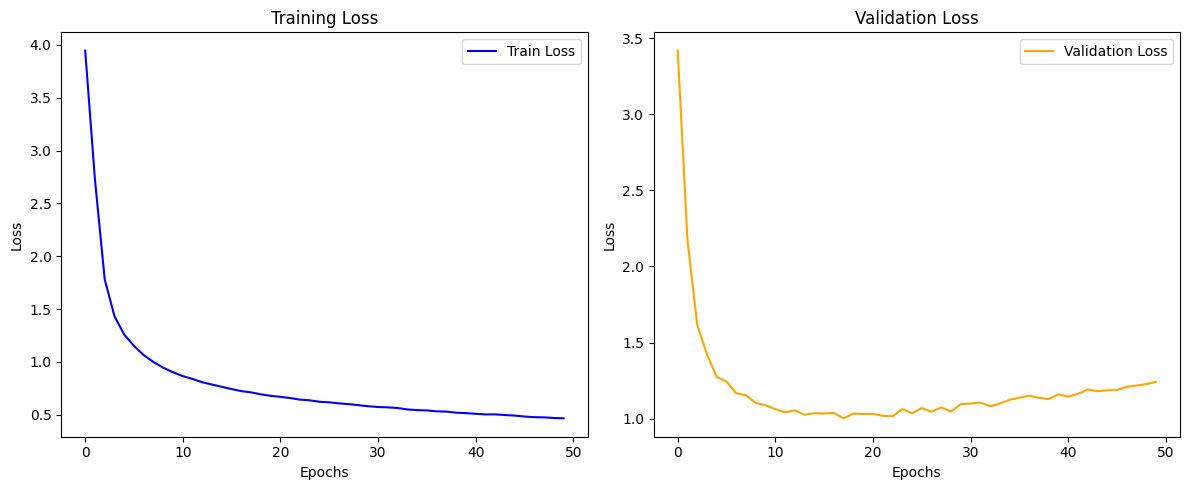
\includegraphics[width=\textwidth]{src/images/figures/OCR_loss_curve.png}
    \caption{Training Loss vs Epochs (\gls{ocr})}
    \label{fig:ocr-training-loss}
\end{figure}

\subsection{OCR Prediction}

% Due to the limitation of unpaid versions of cloud-based services like Google Colab and Lightning \gls{ai}, only 29 training epochs were successfully run. However, the results in those 29 epochs also seem promising as the training loss steadily decreased.
The predictions made by the OCR model for a random sample of test data is shown in \cref{fig:ocr-predictions}. The OCR model accurately recognizes the easily discernible text but is fallible in some cases. However, in this random sample of images, all the problem images (i.e. the ones OCR cannot recognize) are indiscernible to human eyes as well. For instance, the input image samples for GT: D5 and GT: 31 are completely black suggesting a preprocessing or cropping bug rather than a fault in the model.
\begin{figure}[H]
    \centering
    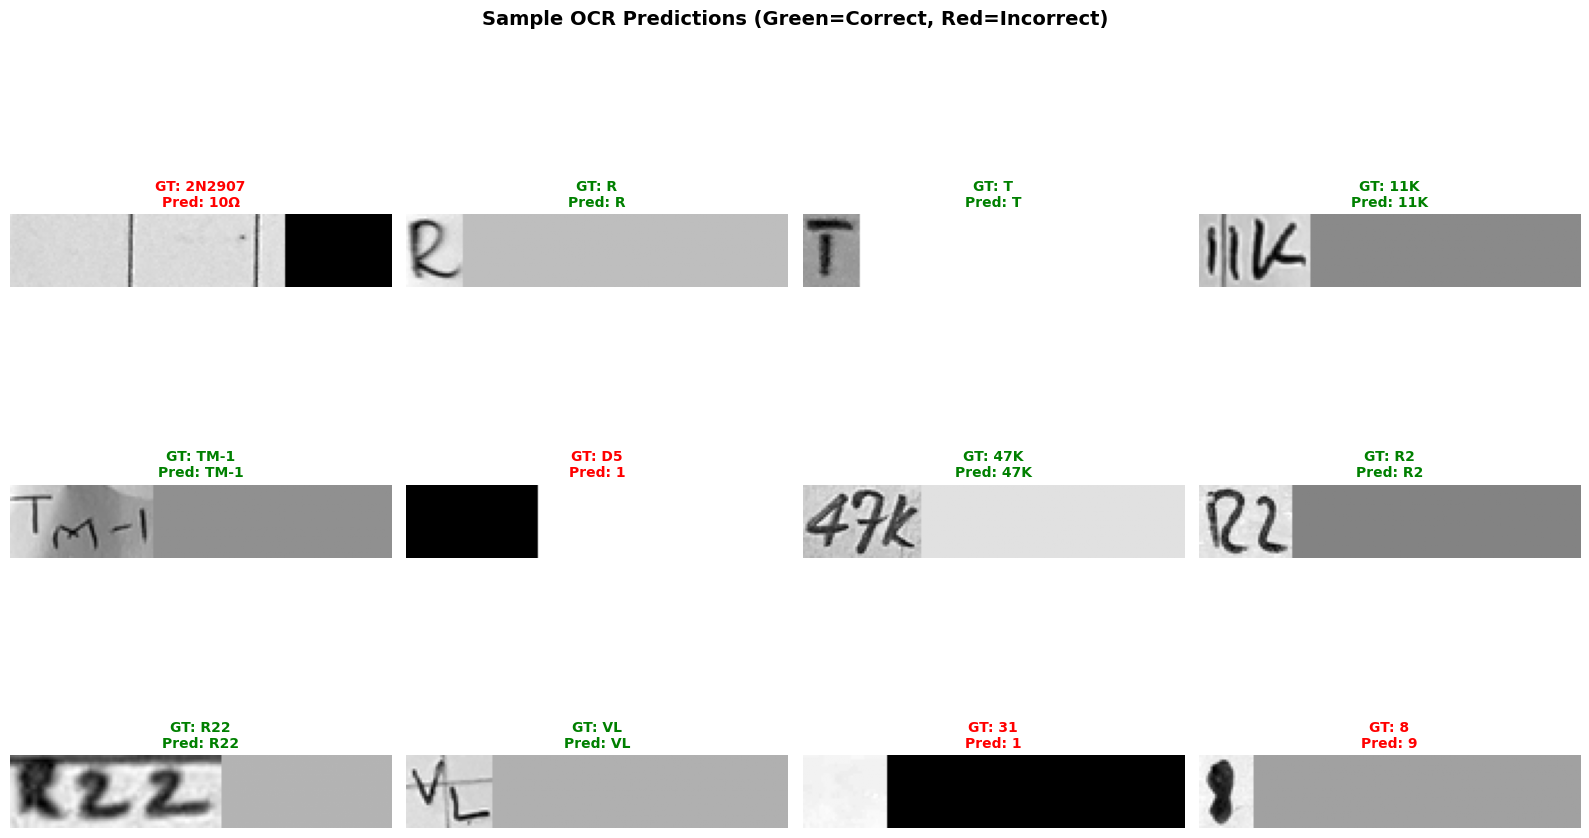
\includegraphics[width=\textwidth]{src/images/figures/ocr_test.png}
    \caption{OCR Model Predictions}
    \label{fig:ocr-predictions}
\end{figure}

\subsection{OCR Performance Analysis}
\cref{fig:ocr-performance-metrics} is a combination of images showing the performance metrics for the OCR model. The accuracy is 65.96\% and while this may seem low, the sample images reveal that accuracy might have taken a hit due to data corruption in the cropping process or preprocessing. Once this bug is somewhat fixed, accuracy is expected to rise. That being said, to improve the accuracy further, the task of refining the model, regardless of data corruption will continue. Likewise, the CER of 0.25 means that on average, 1 out of every 4 characters is predicted incorrectly. However, the histogram shows a notable bump at 1.0 (complete failure) confirming the presence of "garbage" inputs (like black boxes, as seen in the sample images). WER is shown to be 0.34. Its distribution is inherently binary because the model either gets the full component value right (WER being 0) or gets it wrong (WER = 1).
\begin{figure}[H]
    \centering
    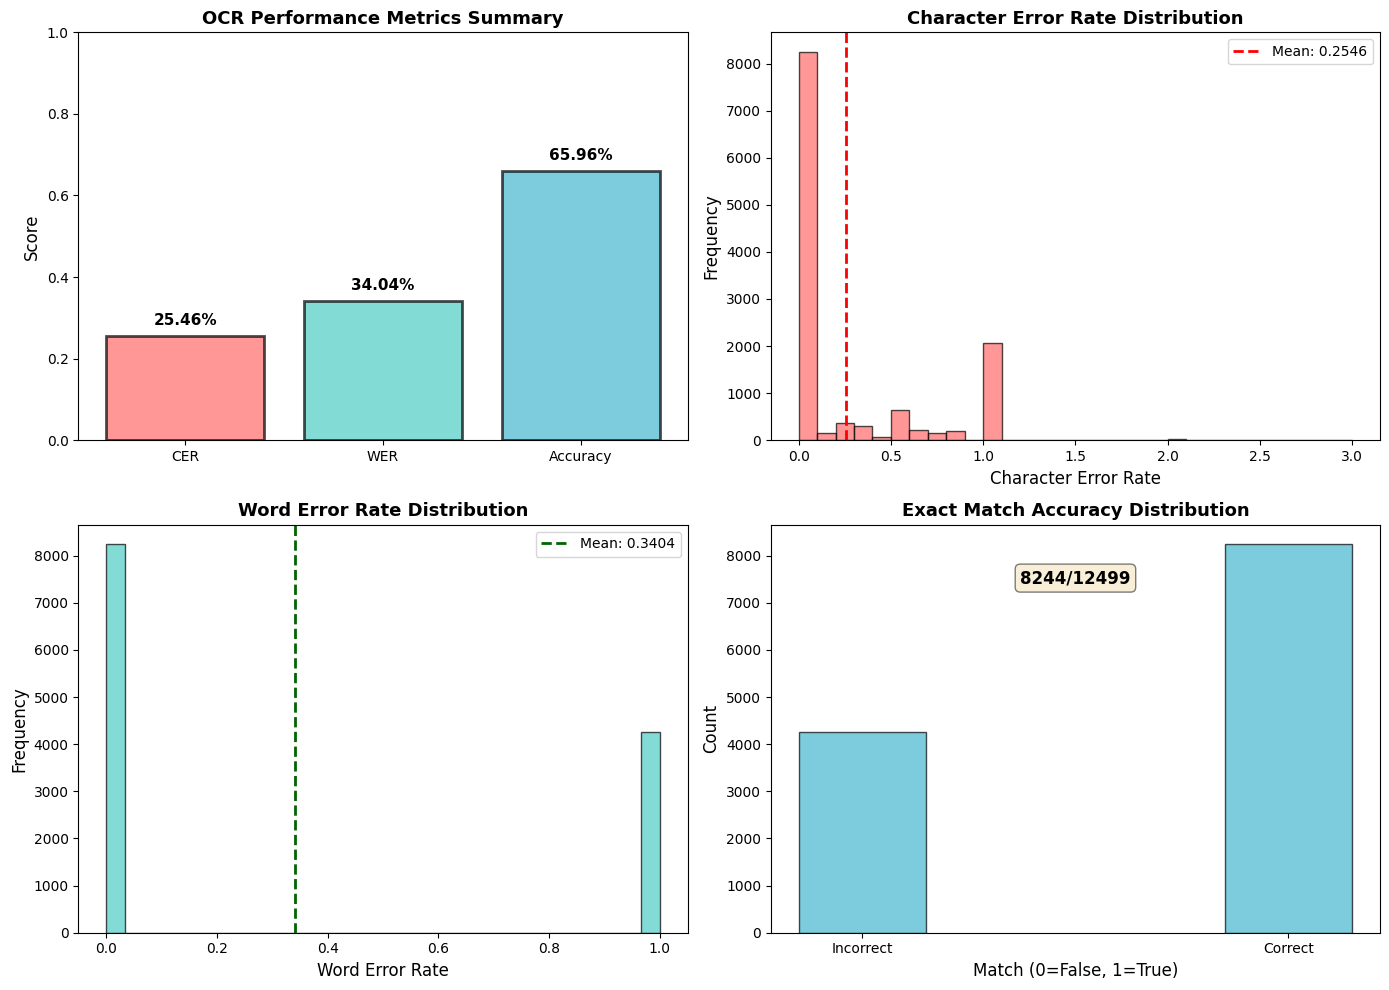
\includegraphics[width=\textwidth]{src/images/figures/cer_wer.png}
    \caption{OCR Performance Metrics and their Distributions}
    \label{fig:ocr-performance-metrics}
\end{figure}

\section{Junction-Based Wire Detection}

This section presents the experimental results obtained from the proposed junction-based wire detection pipeline applied to circuit diagram images. Each processing stage is evaluated independently and supported with quantitative measurements and visual evidence.

\subsection{Input Image and Preprocessing}

The experiment begins with a high-resolution scanned circuit diagram used as the input image. The original image dimensions are reported in terms of width and height in pixels to establish spatial scale consistency throughout the pipeline.

To enhance structural features and suppress background noise, the input image is converted to grayscale. Otsu's global thresholding method is then applied to automatically compute an optimal threshold value that separates foreground circuit elements from the background. The resulting binary image preserves wires, junctions, and components while eliminating illumination variations.

\begin{figure}[H]
    \centering
    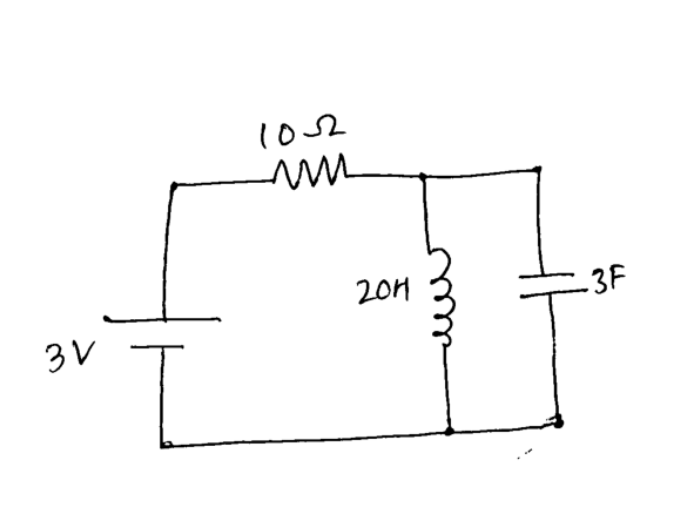
\includegraphics[width=\textwidth]{src/images/figures/otsu_thresholding.png}
    \caption{Otsu's Global Thresholding}
    \label{fig:otsu-thresholding}
\end{figure}

\subsection{Skeletonization}

Morphological skeletonization is applied to the binary image to reduce all wire segments to single pixel-wide centerlines. This transformation significantly reduces the number of foreground pixels while preserving the topological connectivity of the circuit network.

The reduction in foreground pixel count before and after skeletonization is recorded to quantify structural simplification. Despite aggressive thinning, wire continuity and junction connectivity remain intact, making the skeleton suitable for graph-based analysis.

\begin{figure}[H]
    \centering
    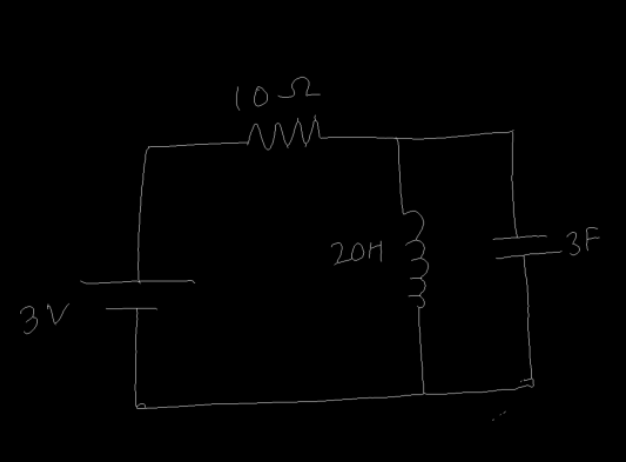
\includegraphics[width=\textwidth]{src/images/figures/skelotonization.png}
    \caption{Skeletonization}
    \label{fig:skeletonization}
\end{figure}

\subsection{Component Removal and Junction Isolation}

Object detection is performed using a trained \gls{yolo} model to identify and localize elements in the circuit diagram. Detected objects are classified as follows: Class 0 corresponds to text annotations, Class 1 corresponds to junctions, and all remaining classes correspond to circuit components.

The total number of detected objects per class is reported. To isolate only the wire network, bounding boxes associated with non-junction classes are removed from the skeleton image. This step eliminates component shapes while preserving junction points and interconnecting wires.

\begin{figure}[H]
    \centering
    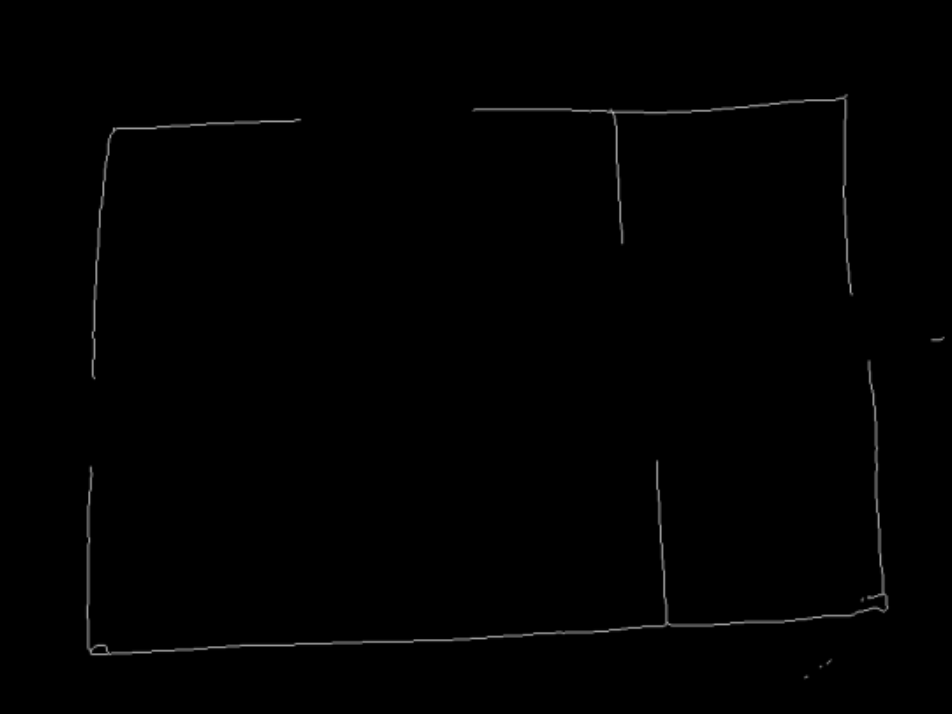
\includegraphics[width=\textwidth]{src/images/figures/component_removal.png}
    \caption{Component Removal}
    \label{fig:component-removal}
\end{figure}

\subsection{Junction Extraction and Wire Classification}

All detected junctions belonging to Class 1 (junctions) are extracted and their coordinates are converted from normalized \gls{yolo} format to pixel coordinates.

Each junction pair is classified based on geometric alignment. Pairs aligned horizontally are labeled as horizontal wires, pairs aligned vertically are labeled as vertical wires, and diagonally aligned pairs are rejected. The total number of accepted and rejected pairs is reported. Sample coordinate transformations from normalized values to pixel coordinates are also presented.

\begin{figure}[H]
    \centering
    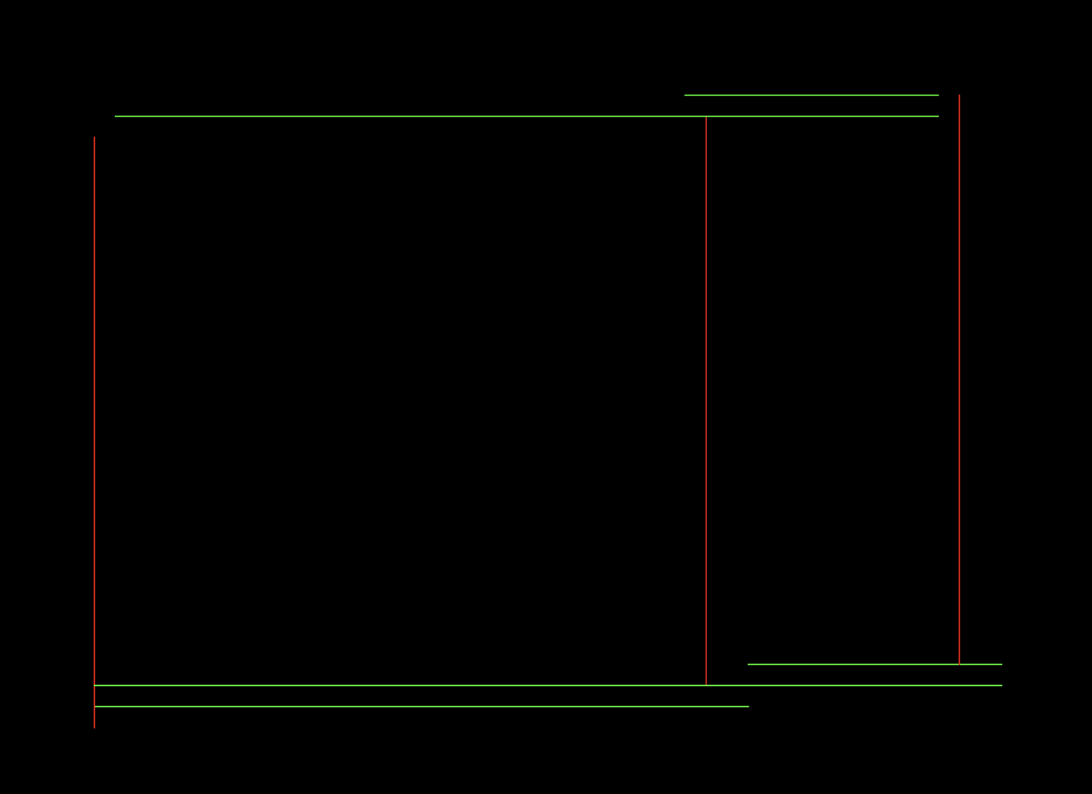
\includegraphics[width=\textwidth]{src/images/figures/wire_classification.png}
    \caption{Wire Classification}
    \label{fig:wire-classification}
\end{figure}

\subsection{Segment Consolidation Through Merging}

Initial wire detection may produce fragmented segments representing portions of the same physical wire. To address this, a merging algorithm is applied based on axis alignment tolerance of 16 pixels and overlapping or adjacent segment conditions.

The total number of raw wire segments before merging and the consolidated count after merging are reported.

\begin{figure}[H]
    \centering
    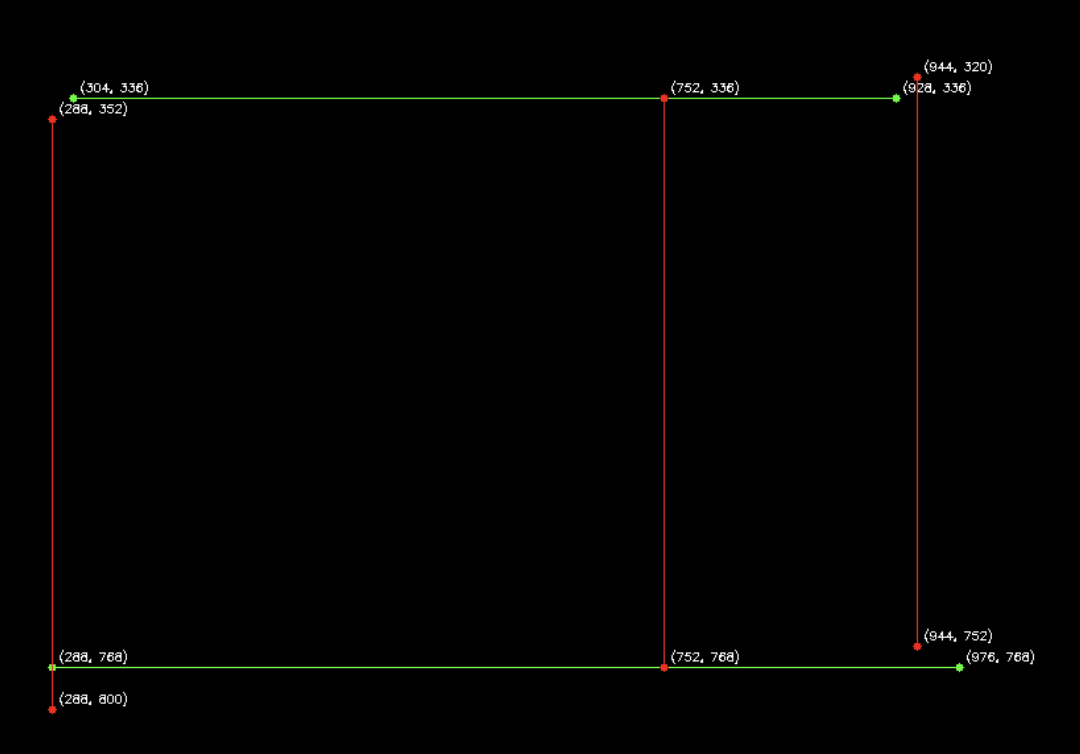
\includegraphics[width=\textwidth]{src/images/figures/segment_consolidation.png}
    \caption{Segment Consolidation Through Merging}
    \label{fig:segment-consolidation}
\end{figure}

\subsection{Component Bounding Box Overlay}

To enhance visualization and verify correct detection, component bounding boxes detected by \gls{yolo} are overlaid on the original circuit diagram. This overlay confirms that all circuit elements have been properly identified and localized, with bounding boxes accurately delineating component boundaries.

\begin{figure}[H]
    \centering
    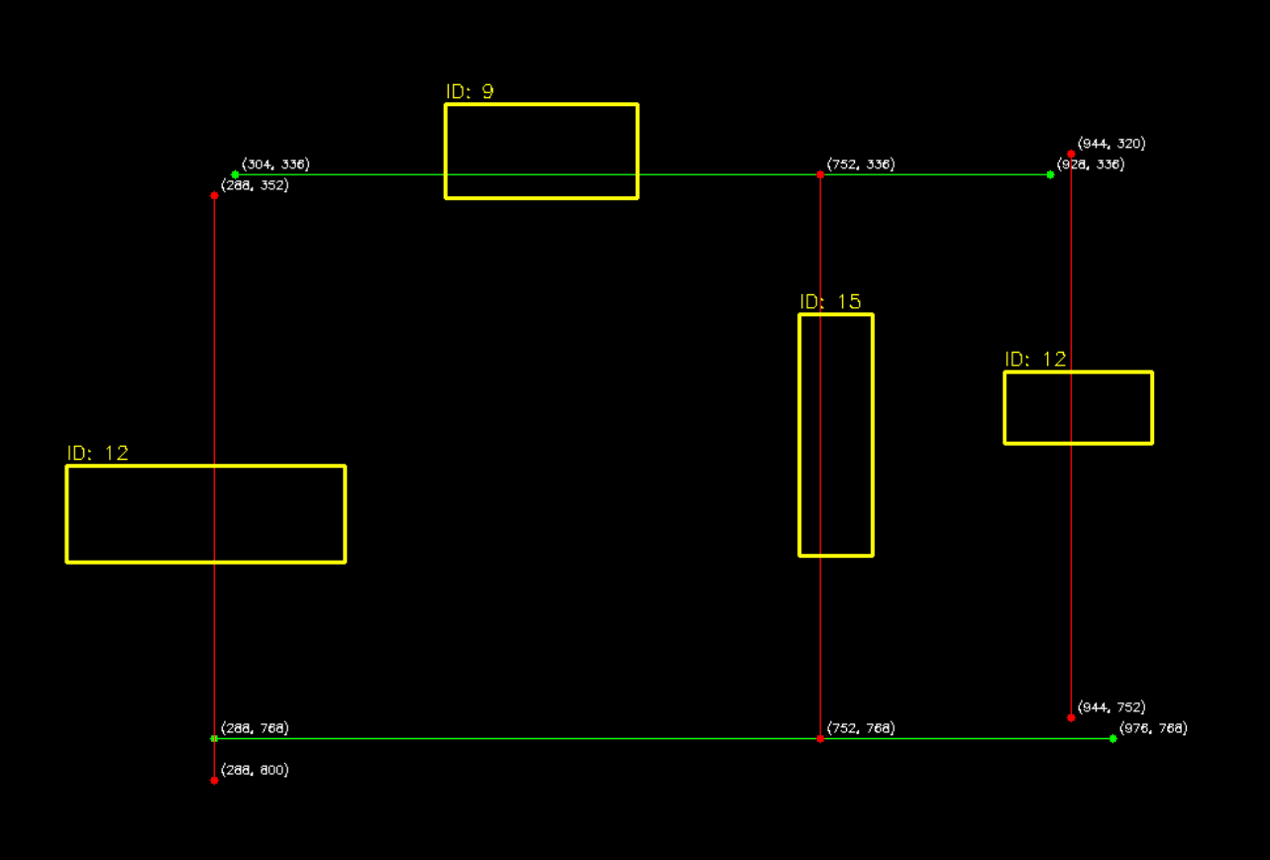
\includegraphics[width=\textwidth]{src/images/figures/bounding_box_overlay.png}
    \caption{Bounding Box Overlay}
    \label{fig:bbox-overlay}
\end{figure}

\subsection{Wire-Component Intersection Detection}

Intersection points between wires and component bounding box edges are computed to identify electrical connectivity. The total number of intersection points is reported along with a directional breakdown for horizontal and vertical wires intersecting specific component edges.

These intersections form the basis for reconstructing circuit connectivity graphs and netlists.

\begin{figure}[H]
    \centering
    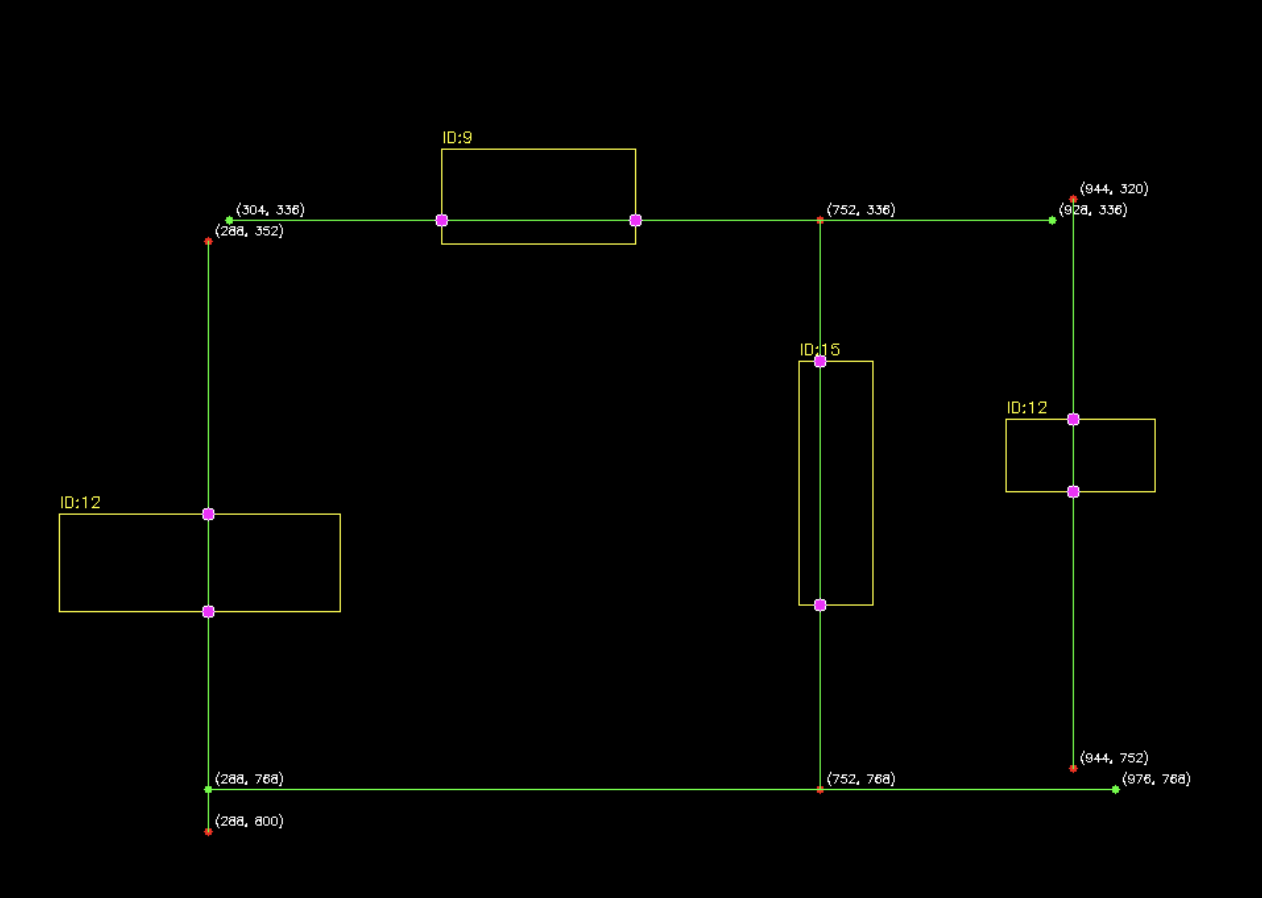
\includegraphics[width=\textwidth]{src/images/figures/wire_component_intersection_detection.png}
    \caption{Wire-Component Intersection Detection}
    \label{fig:wire-component-intersection}
\end{figure}

\section{Line Detection via Path Finding Visualization}

The algorithm produces visual outputs that demonstrate the effectiveness of the endpoint detection and graph construction pipeline. The following subsections present the key visualizations obtained from applying the Multi-Head BFS algorithm to the skeletonized circuit image.

\subsection{Skeletonized Image with Detected Endpoints}

Figure~\ref{fig:skeleton_endpoints} displays the skeletonized image with all detected endpoints overlaid. The skeleton representation captures the one-pixel-wide structure of the circuit lines after morphological processing. Red circles indicate the detected endpoints, which were identified using the bounding box intersection method for line segments and center-snapping for junction points. Green rectangles show the original YOLO bounding boxes used for endpoint localization. This visualization confirms that the endpoint detection algorithm successfully identifies connection points at the boundaries of detected objects.

\begin{figure}[H]
    \centering
    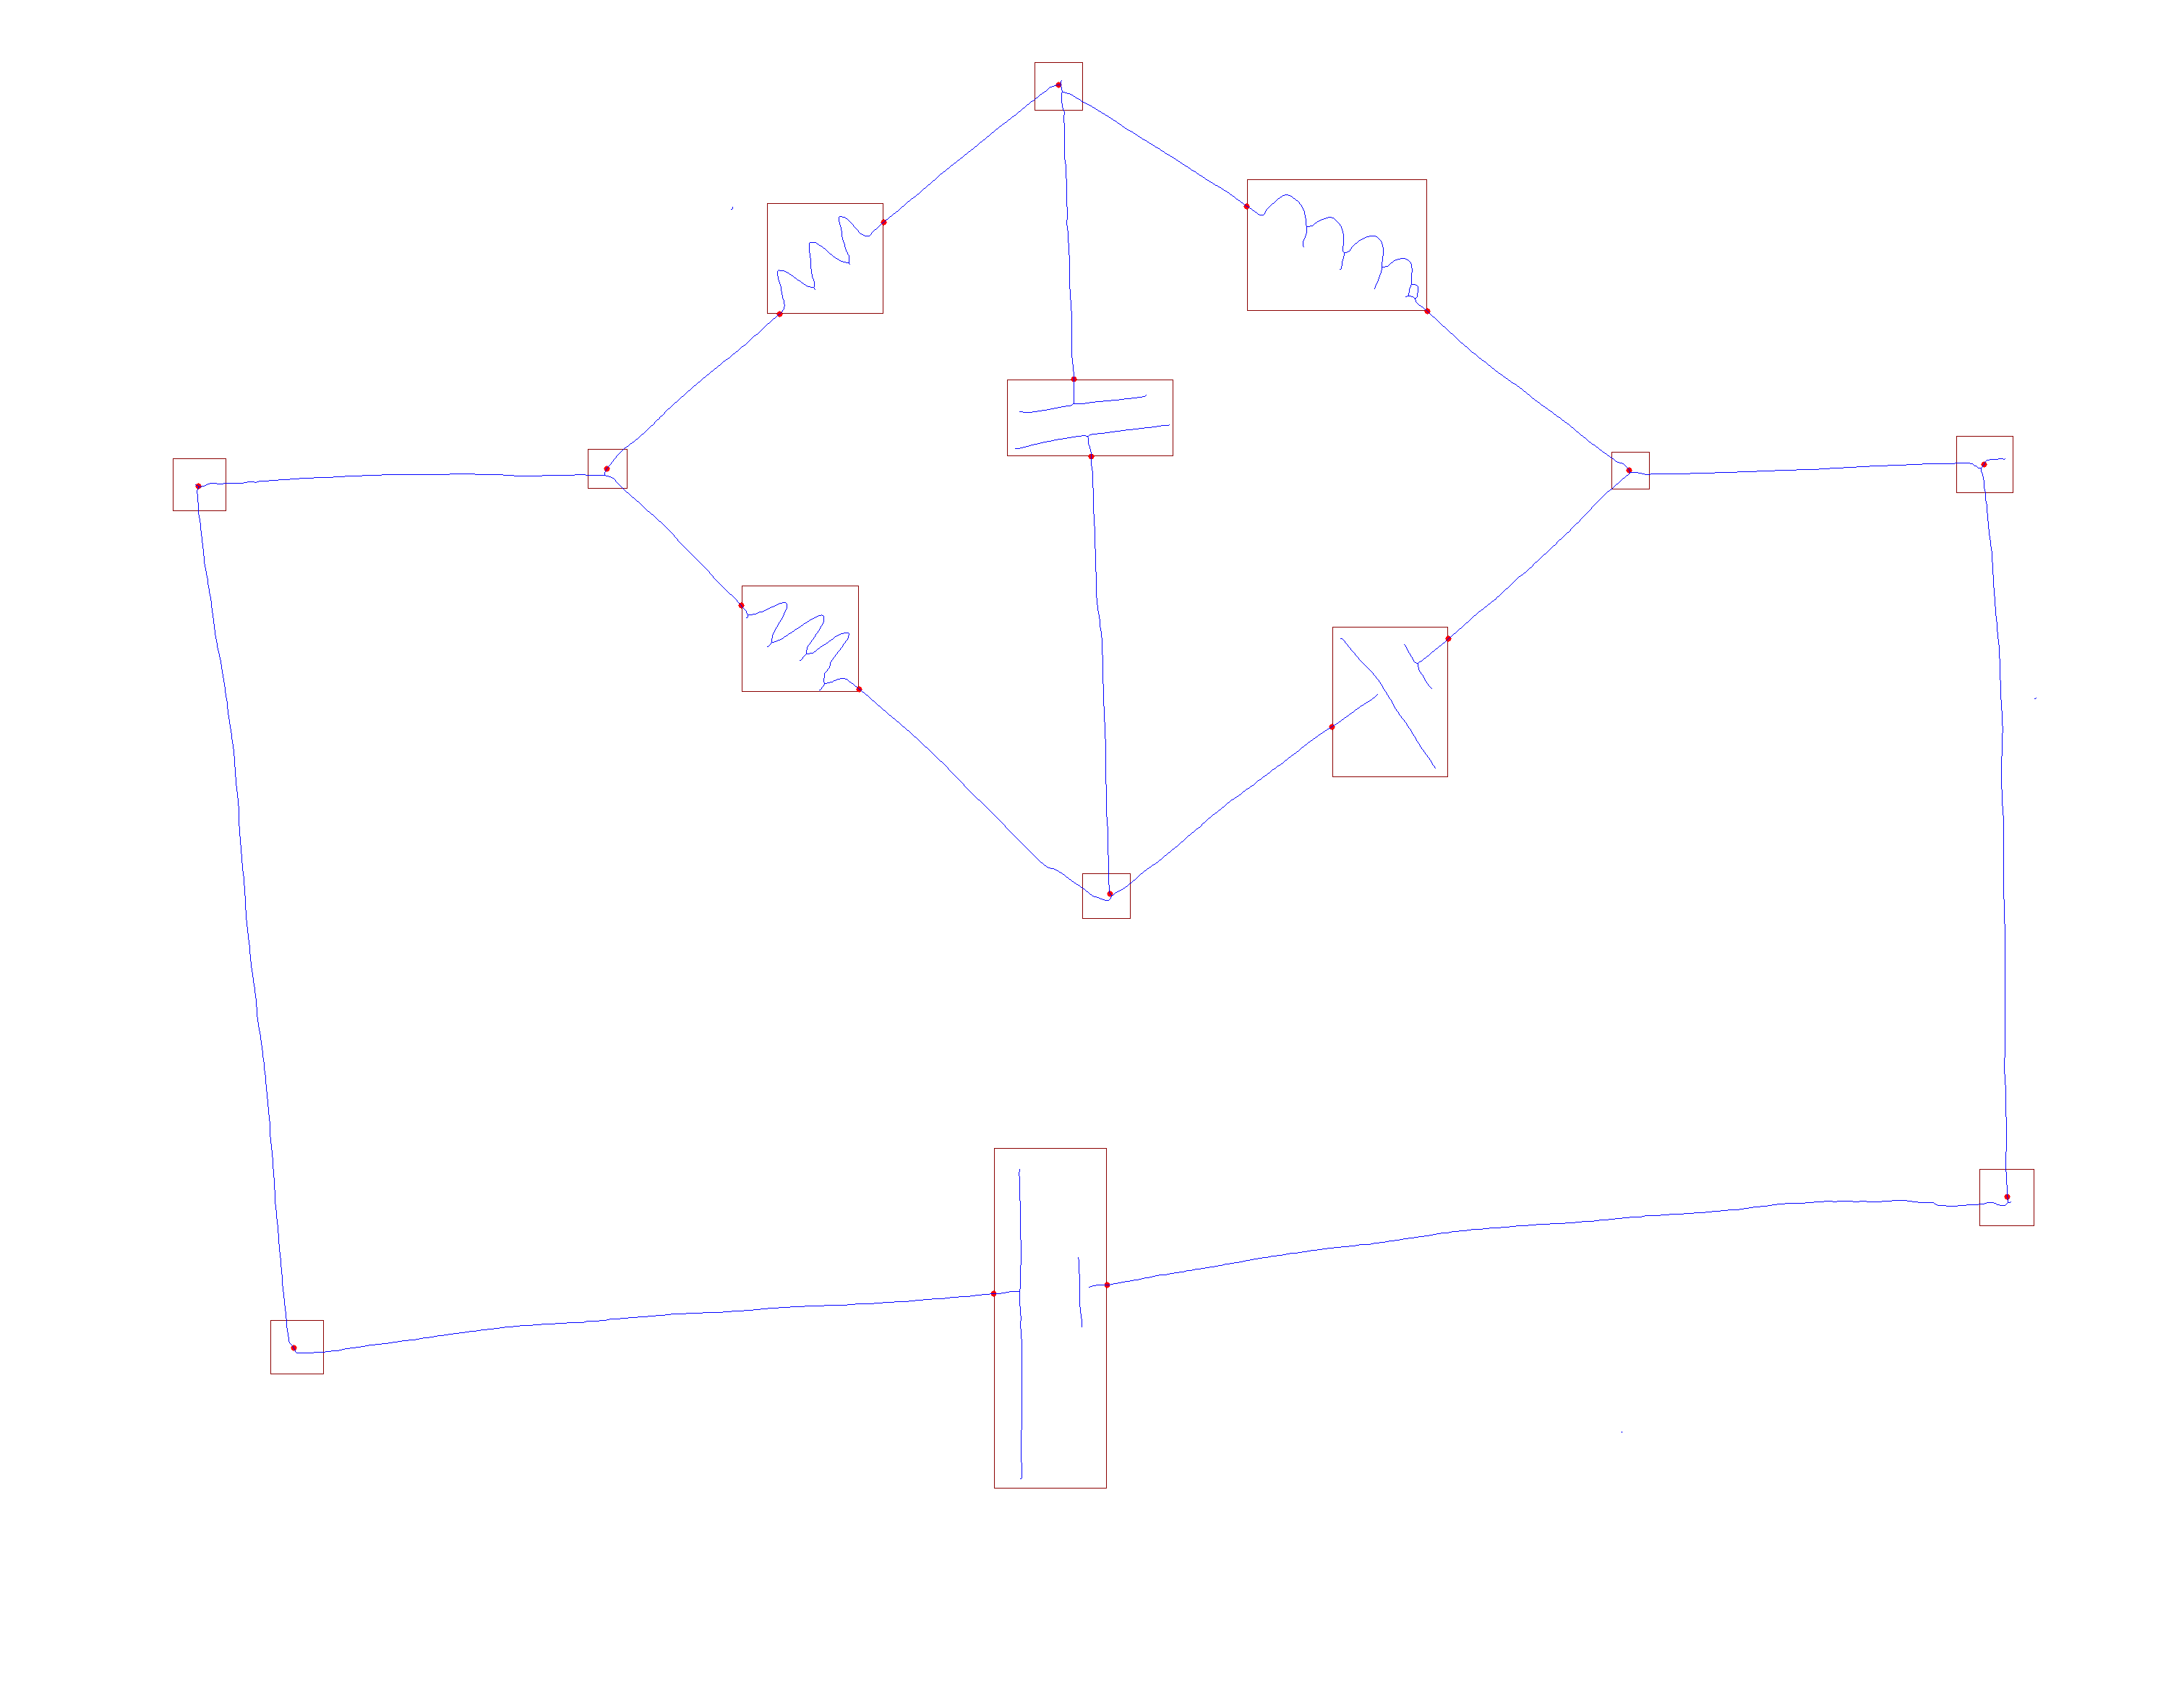
\includegraphics[width=0.8\textwidth]{src/images/figures/skeleton_with_endpoints.png}
    \caption{Skeletonized image with detected endpoints}
    \label{fig:skeleton_endpoints}
\end{figure}

\subsection{Adjacency Graph Visualization}

Figure~\ref{fig:adjacency_graph} presents the final adjacency graph constructed using the Multi-Head BFS algorithm. Each node corresponds to a detected endpoint from the previous stage. Blue lines connecting the nodes represent edges in the graph, indicating skeleton connectivity between endpoints. The graph has been processed to remove self-edges (connections between endpoints belonging to the same detected object), ensuring that only meaningful inter-component connections are preserved. This graph structure enables downstream applications such as circuit topology analysis and netlist extraction.

\begin{figure}[H]
    \centering
    
\includegraphics[width=0.7\textwidth]{src/images/figures/adjacency_graph.png}
    \caption{Adjacency graph constructed using Multi-Head BFS algorithm}
    \label{fig:adjacency_graph}
\end{figure}

\section{Frontend Visualization}

The frontend of the \gls{circuitron} web application provides an interactive environment for circuit design, simulation, and analysis. It enables users to construct electrical circuits using a drag-and-drop schematic editor with grid-based alignment, snap-to-grid functionality, and real-time wire routing. Components such as passive elements, active devices, and sources can be configured through a properties panel that allows precise control over electrical parameters and placement. 

The system integrates simulation controls for transient analysis, allowing users to define time parameters, execute simulations, and visualize results through dynamically rendered voltage-time plots. Measurement probes support real-time signal monitoring with automated computation of key metrics, including maximum, minimum, peak-to-peak range, and \gls{rms} values. Additionally, the frontend supports exporting simulation data and visualizations in standard formats, enabling seamless documentation and further offline analysis.

\begin{figure}[H]
    \centering
    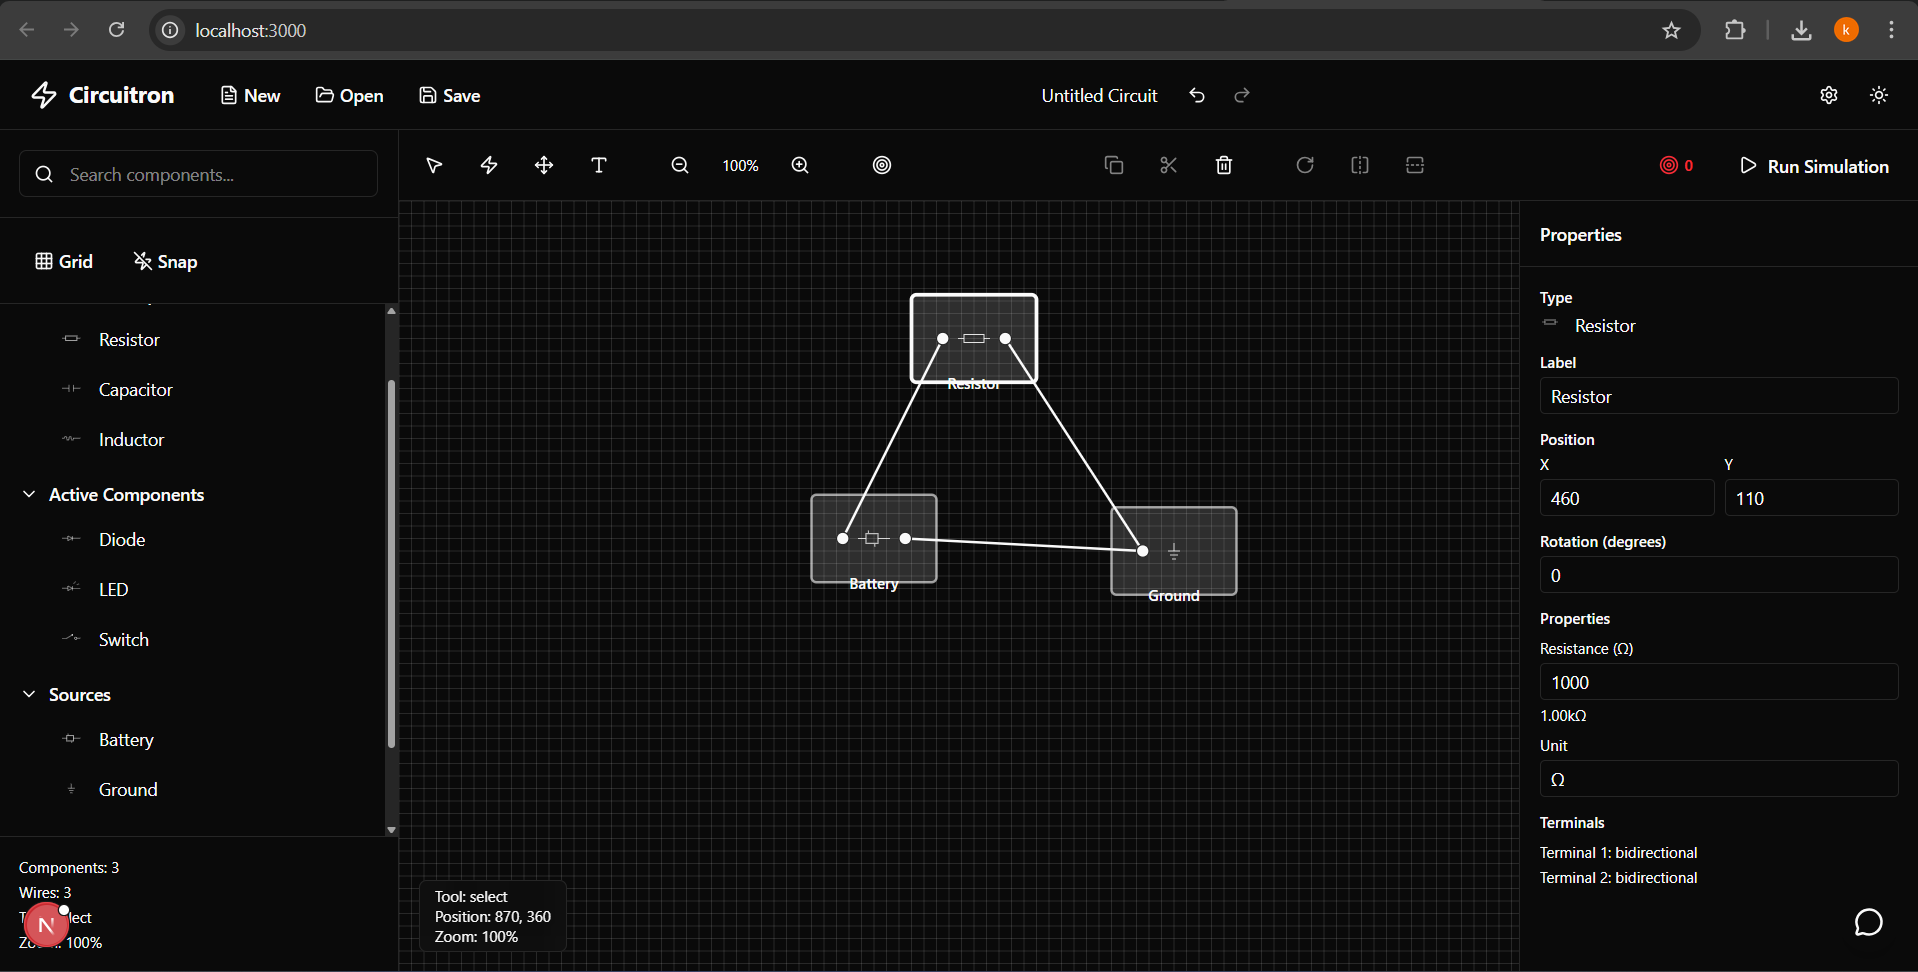
\includegraphics[width=\textwidth]{src/images/figures/frontend_circuit.png}
    \caption{Digitally Drawn Circuit}
    \label{fig:digital-circuit-editor}
\end{figure}

\begin{figure}[H]
    \centering
    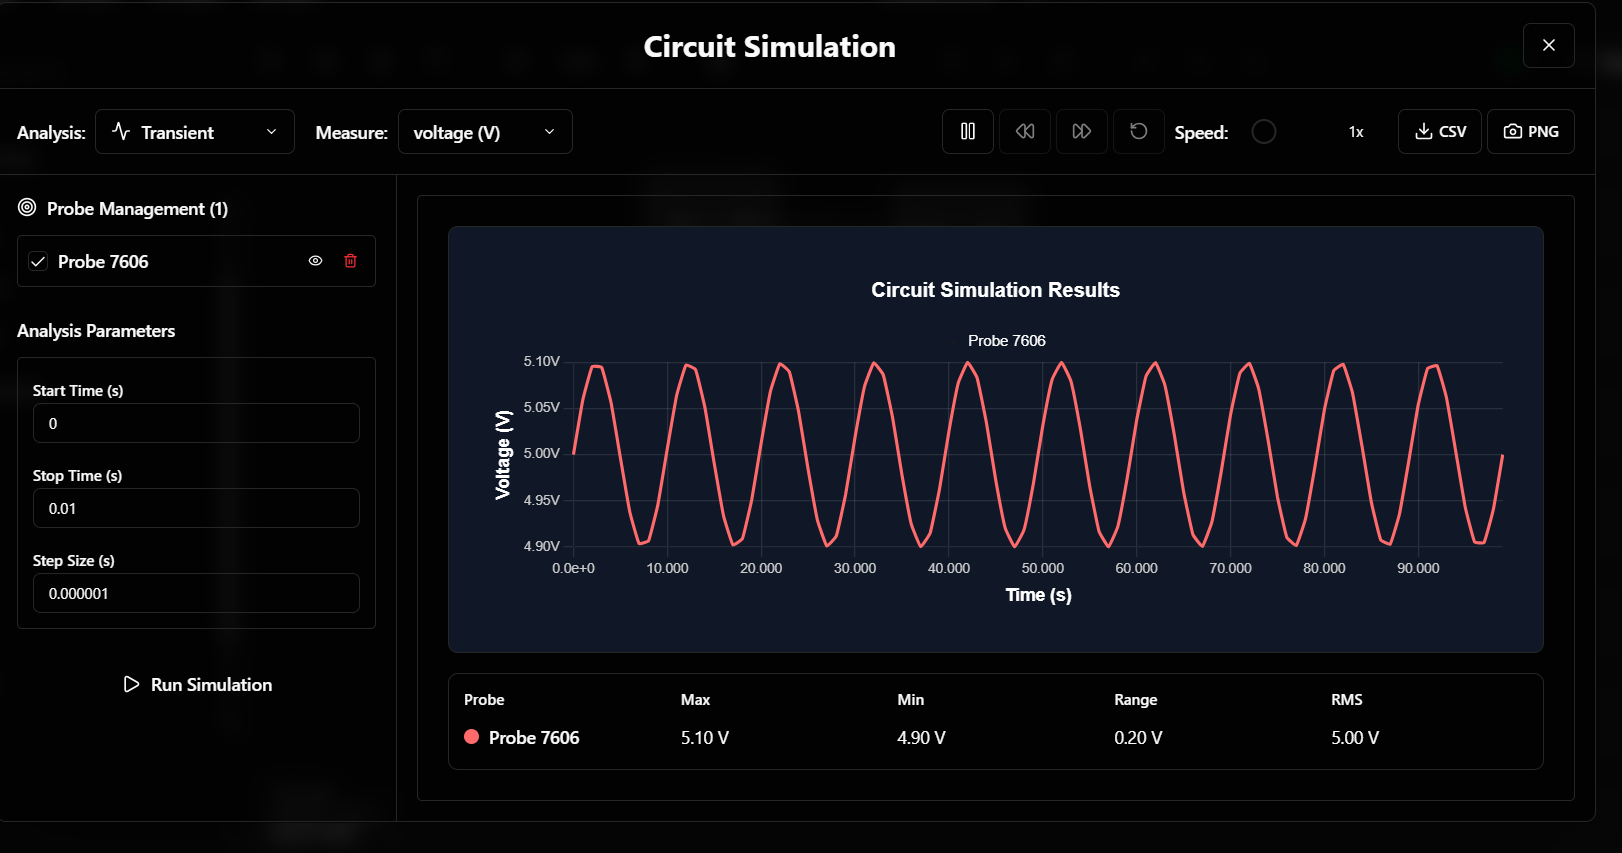
\includegraphics[width=\textwidth]{src/images/figures/frontend_simulation.png}
    \caption{Example Circuit Simulation Result}
    \label{fig:simulation-result}
\end{figure}
